% !TeX spellcheck = hu_HU
% !TeX encoding = UTF-8
% !TeX program = xelatex
% TODO Change language to en_GB (recommended) or en_US for English documents
\documentclass[11pt,a4paper,oneside]{report}             % Single-side
%\documentclass[11pt,a4paper,twoside,openright]{report}  % Duplex

% thanks to http://tex.stackexchange.com/a/47579/71109
\usepackage{ifxetex}
\usepackage{ifluatex}
\newif\ifxetexorluatex % a new conditional starts as false
\ifnum 0\ifxetex 1\fi\ifluatex 1\fi>0
   \xetexorluatextrue
\fi

\ifxetexorluatex
  \usepackage{fontspec}
\else
  \usepackage[T1]{fontenc}
  \usepackage[utf8]{inputenc}
  \usepackage[lighttt]{lmodern}
\fi

\usepackage[english,magyar]{babel} % Alapértelmezés szerint utoljára definiált nyelv lesz aktív, de később külön beállítjuk az aktív nyelvet.

%\usepackage{cmap}
\usepackage{amsfonts,amsmath,amssymb} % Mathematical symbols.
%\usepackage[ruled,boxed,resetcount,linesnumbered]{algorithm2e} % For pseudocodes. % beware: this is not compatible with LuaLaTeX, see http://tex.stackexchange.com/questions/34814/lualatex-and-algorithm2e
\usepackage{booktabs} % For publication quality tables for LaTeX
\usepackage{graphicx}

%\usepackage{fancyhdr}
%\usepackage{lastpage}

\usepackage{anysize}
%\usepackage{sectsty}
\usepackage{setspace} % For setting line spacing

\usepackage[unicode]{hyperref} % For hyperlinks in the generated document.
\usepackage{xcolor}
\usepackage{listings} % For source code snippets.

\usepackage[amsmath,thmmarks]{ntheorem} % Theorem-like environments.

\usepackage[hang]{caption}
\usepackage{float}

\singlespacing

\newcommand{\selecthungarian}{
	\selectlanguage{magyar}
	\setlength{\parindent}{2em}
	\setlength{\parskip}{0em}
	\frenchspacing
}

\newcommand{\selectenglish}{
	\selectlanguage{english}
	\setlength{\parindent}{0em}
	\setlength{\parskip}{0.5em}
	\nonfrenchspacing
	\renewcommand{\figureautorefname}{Figure}
	\renewcommand{\tableautorefname}{Table}
	\renewcommand{\partautorefname}{Part}
	\renewcommand{\chapterautorefname}{Chapter}
	\renewcommand{\sectionautorefname}{Section}
	\renewcommand{\subsectionautorefname}{Section}
	\renewcommand{\subsubsectionautorefname}{Section}
}


%TODO Set the main variables
\newcommand{\vikszerzoVezeteknev}{Dobosy}
\newcommand{\vikszerzoKeresztnev}{Kristóf}
\newcommand{\vikkonzulensA}{Búr Márton} % Első konzulens neve
\newcommand{\vikkonzulensB}{Szárnyas Gábor} % Második konzulens neve; hagyd üresen, ha egy konzulensed van.
\newcommand{\vikcim}{Gráflekérdező motor teljesítménytesztelése modellvalidációs problémákra} % Cím
\newcommand{\viktanszek}{\bmemit} % Tanszék
\newcommand{\vikdoktipus}{\bsc} % Dokumentum típusa (\bsc, \msc)

\input{include/tdk-variables}
\newcommand{\szerzoMeta}{\vikszerzoVezeteknev{} \vikszerzoKeresztnev} % egy szerző esetén
%\newcommand{\szerzoMeta}{\vikszerzoVezeteknev{} \vikszerzoKeresztnev, \tdkszerzoB} % két szerző esetén

%TODO Language configuration -- choose one
% Beállítások magyar nyelvű dolgozathoz
%--------------------------------------------------------------------------------------
% Elnevezések
%--------------------------------------------------------------------------------------
\newcommand{\bme}{Budapesti Műszaki és Gazdaságtudományi Egyetem}
\newcommand{\vik}{Villamosmérnöki és Informatikai Kar}

\newcommand{\bmemit}{Méréstechnika és Információs Rendszerek Tanszék}

\newcommand{\keszitette}{Készítette}
\newcommand{\konzulens}{Konzulens}

\newcommand{\bsc}{Szakdolgozat}
\newcommand{\msc}{Diplomaterv}
\newcommand{\bsconlab}{BSc Önálló laboratórium}
\newcommand{\msconlabi}{MSc Önálló laboratórium 1.}
\newcommand{\msconlabii}{MSc Önálló laboratórium 2.}

\newcommand{\pelda}{Példa}
\newcommand{\definicio}{Definíció}
\newcommand{\tetel}{Tétel}

\newcommand{\bevezetes}{Bevezetés}
\newcommand{\koszonetnyilvanitas}{Köszönetnyilvánítás}
\newcommand{\abrakjegyzeke}{Ábrák jegyzéke}
\newcommand{\tablazatokjegyzeke}{Táblázatok jegyzéke}
\newcommand{\irodalomjegyzek}{Irodalomjegyzék}
\newcommand{\fuggelek}{Függelék}

\newcommand{\szerzo}{\vikszerzoVezeteknev{} \vikszerzoKeresztnev}

\newcommand{\selectthesislanguage}{\selecthungarian}

\bibliographystyle{huplain}

\def\lstlistingname{lista}

\newcommand{\appendixnumber}{6}  % a fofejezet-szamlalo az angol ABC 6. betuje (F) lesz

\newcommand{\Csh}{C\#}
\newcommand{\cpp}{C\texttt{++}}
% Settings for English documents
%\input{include/thesis-en}

\input{include/preamble}

%--------------------------------------------------------------------------------------
% Table of contents and the main text
%--------------------------------------------------------------------------------------
\begin{document}

%TODO These define guidelines -- remove these
%~~~~~~~~~~~~~~~~~~~~~~~~~~~~~~~~~~~~~~~~~~~~~~~~~~~~~~~~~~~~~~~~~~~~~~~~~~~~~~~~~~~~~~
\include{include/guideline}
\include{include/project}

\selectthesislanguage

%TODO Titlepage -- choose one from below
%~~~~~~~~~~~~~~~~~~~~~~~~~~~~~~~~~~~~~~~~~~~~~~~~~~~~~~~~~~~~~~~~~~~~~~~~~~~~~~~~~~~~~~
\include{include/titlepage}		   % Szakdolgozat/Diplomaterv címlap
%\include{include/titlepage-tdk}	% TDK címlap
%\include{include/titlepage-otdk}   % OTDK címlap


% Table of Contents
%~~~~~~~~~~~~~~~~~~~~~~~~~~~~~~~~~~~~~~~~~~~~~~~~~~~~~~~~~~~~~~~~~~~~~~~~~~~~~~~~~~~~~~
\tableofcontents\vfill


% Declaration and Abstract
%~~~~~~~~~~~~~~~~~~~~~~~~~~~~~~~~~~~~~~~~~~~~~~~~~~~~~~~~~~~~~~~~~~~~~~~~~~~~~~~~~~~~~~
\selectlanguage{magyar}
\pagenumbering{gobble}
%--------------------------------------------------------------------------------------
% Nyilatkozat
%--------------------------------------------------------------------------------------
\begin{center}
\large
\textbf{HALLGATÓI NYILATKOZAT}\\
\end{center}

Alulírott \emph{\vikszerzoVezeteknev{} \vikszerzoKeresztnev}, szigorló hallgató kijelentem, hogy ezt a szakdolgozatot meg nem engedett segítség nélkül, saját magam készítettem, csak a megadott forrásokat (szakirodalom, eszközök stb.) használtam fel. Minden olyan részt, melyet szó szerint, vagy azonos értelemben, de átfogalmazva más forrásból átvettem, egyértelműen, a forrás megadásával megjelöltem.

Hozzájárulok, hogy a jelen munkám alapadatait (szerző(k), cím, angol és magyar nyelvű tartalmi kivonat, készítés éve, konzulens(ek) neve) a BME VIK nyilvánosan hozzáférhető elektronikus formában, a munka teljes szövegét pedig az egyetem belső hálózatán keresztül (vagy autentikált felhasználók számára) közzétegye. Kijelentem, hogy a benyújtott munka és annak elektronikus verziója megegyezik. Dékáni engedéllyel titkosított diplomatervek esetén a dolgozat szövege csak 3 év eltelte után válik hozzáférhetővé.

\begin{flushleft}
\vspace*{1cm}
Budapest, \today
\end{flushleft}

\begin{flushright}
 \vspace*{1cm}
 \makebox[7cm]{\rule{6cm}{.4pt}}\\
 \makebox[7cm]{\emph{\vikszerzoVezeteknev{} \vikszerzoKeresztnev}}\\
 \makebox[7cm]{hallgató}
\end{flushright}
\thispagestyle{empty}

\vfill
\clearpage
\thispagestyle{empty} % an empty page

\selectthesislanguage
 %TODO Hallgatói nyilatkozat -- TDK és OTDK esetén törlendő!
\pagenumbering{roman}
\setcounter{page}{1}

\selecthungarian

%----------------------------------------------------------------------------
% Abstract in Hungarian
%----------------------------------------------------------------------------
\chapter*{Kivonat}\addcontentsline{toc}{chapter}{Kivonat}

Modell-vezérelt fejlesztési folyamatoknál a modellt valamilyen adatkezelő-eszközön tároljuk és ezen keresztül végzünk rajta műveleteket. Az eszközök teljesítménye meghatározza a teljes fejlesztés idejét, ezáltal elengedhetetlen kérdés a különböző elérhető eszközök teljesítményének mérése és összehasonlítása.

Emellett a modell-vezérelt fejlesztésnél jól-formáltság ellenőrzése fontos feladat. A modellre meghatározott kényszerek validációja különböző eszközökön végzett lekérdezések segítségével történik. Továbbá a fejlesztési folyamat során a modellbe hibák injektálódnak és javítódnak. Az eszközök teljesítményét össze lehet hasonlítani az alapján, hogy ezeket a műveleteket mennyi idő alatt végzik el. Egy ilyen teljesítménymérést végez a Train Benchmark projekt egy vasúti elemekből álló modellen. A dolgozat írásakor a Train Benchmark keretrendszer már elkészült tíz eszközre.

Jelen szakdolgozat ismerteti a Train Benchmark keretrendszer működését, majd két gráfadatbázis-kezelő eszközön elvégzett mérés eredményét rögzíti. Továbbá a Graph Engine nevű Microsoft által fejlesztett eszköz működését bemutatja, illetve az erre implementált teljesítménymérést kiértékeli és összehasonlítja a két rögzített eredménnyel. Emellett egy általános képet ad a gráfalapú adatbázisok sajátosságairól. Végül összefoglalja a Graph Engine előnyeit és hátrányait.

\vfill
\selectenglish


%----------------------------------------------------------------------------
% Abstract in English
%----------------------------------------------------------------------------
\chapter*{Abstract}\addcontentsline{toc}{chapter}{Abstract}

Verifying the well-formedness of a model is highly important in model-driven developments. The validation of predetermined constraints is run by querying with different tools. In addition, faults get injected and corrected into the model during the development process. The tools can be compared based on how much time they need to be finished. The Train Benchmark project concentrates such an evaluation on model which consists of railway elements. The Train Benchmark has already been implemented for ten tools. This thesis is about to describe how the Train Benchmark operates. It also shows the performing process of the benchmarking on two graph database tools. Moreover, it demonstrates an additional tool, named Graph Engine, which was developed by Microsoft. Afterwards, it assesses the benchmarking of the Graph Engine and compares it with the results of the other two tools. Besides, it gives a general summary of the particularity of graph databases. In the end, it sums up the advantages and disadvantages of the Graph Engine.

\vfill
\selectthesislanguage

\newcounter{romanPage}
\setcounter{romanPage}{\value{page}}
\stepcounter{romanPage}    %TODO Összefoglaló -- TDK és OTDK esetén nem kötelező


% The main part of the thesis
%~~~~~~~~~~~~~~~~~~~~~~~~~~~~~~~~~~~~~~~~~~~~~~~~~~~~~~~~~~~~~~~~~~~~~~~~~~~~~~~~~~~~~~
\pagenumbering{arabic}

%TODO import your own content
%----------------------------------------------------------------------------
\chapter{\bevezetes}
%----------------------------------------------------------------------------

Számos adatbázis-kezelő rendszer van a világon. A teljesítmény kulcsfontosságú jelentőséggel bír, főleg, amikor nagyméretű adatbázisokról van szó. Emiatt felmerül a kérdés, hogy sorba lehet-e őket rendezni valamilyen objektív mérce alapján. A problémák sokrétűsége azt mutatja, hogy a felhasználási terület általában nagymértékben befolyásolja az eredményt. Emellett az adatbázis-kezelő rendszereket sokféleképp kategóriába is lehet sorolni, például a matematikai modell vagy a lekérdezés nyelve alapján. Az egy kategóriába eső rendszereket általában könnyebb összehasonlítani, mint olyanokat, amik külön kategóriába esnek. Ezek a problémák szinte lehetetlen feladattá tesznek egy általános összehasonlítást. Észszerűen ezért a legtöbb teljesítménymérés egy bizonyos fajta problémára összpontosul. Egy ilyen feladat lehet a modell-validálás, melynek célja, hogy adott modellen (melyet az adatbázisban tárolunk) megkövetelt kényszereket ellenőrizzen. Ez rendkívül fontos egy fejlesztési folyamat során, mivel visszajelzést ad a programozónak és/vagy a felhasználónak a modell helyességéről. A Train Benchmark célja egy ilyen folyamat szimulálása több adatbázisrendszeren és a teljesítményük mérése, annak kiértékelése.

%meg lett valósítva nem túl szép
A Train Benchmark több adatbázis-kezelő rendszerre már meg lett valósítva. Jelen dolgozat célja egy modern adatbázis-kezelő tesztelésének implementálása, a Train Benchmark két adatbázisrendszer-tesztjének futtatása Windows operációs rendszeren és a kapott eredmények összehasonlítása. A kiválasztott adatbáziskezelő-rendszer a Microsoft által fejlesztett Graph Engine.

\section{A dolgozat felépítése}

Az elkészült dolgozat a következő részekből épül fel:

A 2. fejezetben a Train Benchmark modelljének a működésének elvét mutatjuk be. Kezdve a Train Benchmarkban használt modell elemeivel, közöttük lévő kapcsolattal, majd a megfogalmazott kényszerek részletezésével, aztán a fejlesztési folyamat forgatókönyve, végül pedig azon környezetek (Jena, RDF4J) rövid bemutatása következik, melyeknek tesztjét lefuttattuk.

A 3. fejezet az adatbázisrendszerek egy típusáról, a gráfadatbázisokról szól. Egy egyszerű példán keresztül megmutatjuk, hogy adott esetben miért lehet gyorsabb és jobb a relációs adatbázisrendszereknél.

A 4. fejezet a Graph Engine nevű gráfadatbázis-rendszer felépítését és működését taglalja. A 3. fejezetben található példán keresztül mutatjuk be, hogy milyen módon kell használni.

Az 5. fejezetben az általunk elkészített tesztelőprogram implementációját részletezzük. Rövid forráskódokat kiragadva általánosan bemutatjuk, hogy hogyan épül fel. Kiegészítve a Train Benchmarkhoz már elkészült tesztek Windows operációs rendszeren való futtatási problémáinak megoldásával, illetve a fejlesztés során felmerülő nehézségekre való válaszok okainak indoklásával.

%TODO: utolsó két fejezethez tartozó bevezető

A 6. fejezet a tesztek futtatása után kapott eredmények kiértékelését foglalja magában.

A 7. fejezet összefoglalja a dolgozat során elvégzett munkát
%----------------------------------------------------------------------------
\chapter{A Train Benchmark}
%----------------------------------------------------------------------------
Egy számítógép által elvégzendő felügyeleti, esetleg irányítási feladat elvégzéséhez általában elkészítünk egy modellt, ami a rendszer egy leírása. A modell a világ képzelt vagy valós elemeit és ezeknek a számunkra fontos tulajdonságait írja le. Egy valós modellezési folyamat során olyan komplex maga a valóság is, hogy képtelenség hiba nélkül elsőre előállítani a modellt. A hibák ellenőrzésére általában ki szoktak kötni kényszereket, melyek olyan megkötések, amik nem lehetséges eseteket zárnak ki. Egy valós fejlesztési folyamat során megalkotnak egy modellt, ami általában nem hibamentes, az előre meghatározott kényszerek sem teljesülnek rájuk. Utána minden fejlesztési szakaszban kijavítanak néhány hibát, majd újraellenőrzik a modellt és ezt ciklikusan folytatják addig, amíg minden kényszernek meg nem felel. Sok esetben ezzel párhuzamosan történik a modell bővítése is, ami újabb hibákat eredményez.

A modell elemeit minden esetben valamilyen adatbázisban tárolják. Mivel az adatokon végzett műveletek többségét támogatják elterjedt adatbázis-kezelő szoftverek, ezért többnyire a fejlesztési folyamatban egy ilyen szoftvert választanak. A Train Benchmark egy ilyen folyamat különböző adatbázis-kezelő szoftvereken való lefuttatását hasonlítja össze, ezzel szimulálva a valós fejlesztést és célja a szoftverek teljesítményének összehasonlítása.

\section{A modell felépítése}

A Train Benchmark egy vasúti pályának az elemeit, azok tulajdonságait használja fel egy valós probléma szimulálására. A modell osztályokból épül fel, amik meghatározzák az adott elemnek az általunk fontos tulajdonságok összességét, ezeket tároljuk. Ezek az osztályok a következők:
\begin{itemize}
	\item \emph{RailwayElement}: Minden osztály ennek az osztálynak a leszármazottja. Egyetlen közös tulajdonságot, az egyedi azonosítót tartalmazza.
	\item \emph{Semaphore}: Jelzi a vonatnak, hogy az adott útszakaszon áthaladhat-e. Az aktuális állapotát tároljuk. (A továbbiakban: szemafor)
	\item \emph{TrackElement}: A sípálya legkisebb számunkra fontos alkotóelemei, a \emph{Segment} és a \emph{Switch} ősosztálya.
	\item \emph{Segment}: Az útnak egy kisebb része, ami már megfigyelhető szenzorok által. A modellben szereplő tulajdonsága a hossza. (A továbbiakban: útszakasz)
	\item \emph{Switch}: Két útszakasz között helyezkedik el és meghatározza azt, hogy merre halad tovább a vonat, amikor ideér. (A továbbiakban váltó)
	\item \emph{Route}: Egy vasúti sínpár szakasza két szemafor között. útszakaszokból és váltókból áll össze. Azt tároljuk róla, hogy aktív-e, azaz, hogy az összes váltó olyan állásban van, hogy a vonat ezen az útvonalon halad végig. (A továbbiakban: út)
	\item \emph{Region}: Szenzorokat, útszakaszokat és váltókat magába foglaló konténer. (A továbbiakban régió)
	\item \emph{RailwayContainer}: Utakat és a régiókat tartalmazó konténer.
	\item \emph{Sensor}: A hozzá tartozó útszakaszokat, illetve váltókat monitorozza. (A továbbiakban: szenzor)
	\item \emph{SwitchPosition}: A váltó az úthoz mért relatív állását mutatja, azaz, hogy a váltónak merre kell állnia, hogy a szegmenseken végighaladó vonat az adott úton haladjon. 
\end{itemize}

\begin{figure}
	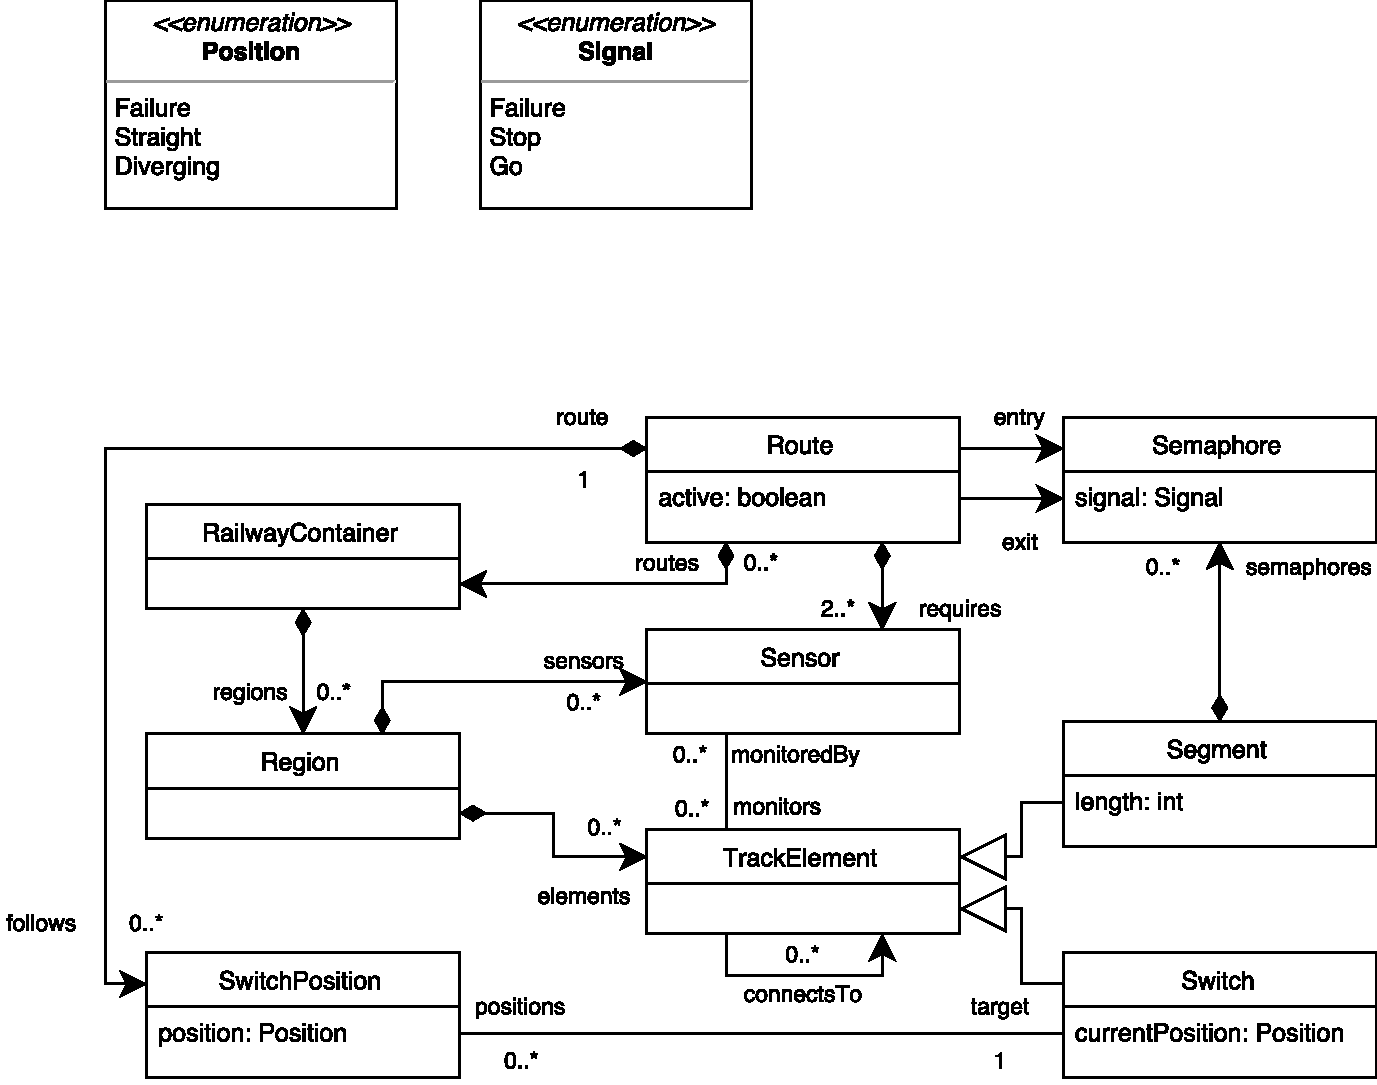
\includegraphics[width=\linewidth, keepaspectratio]{figures/model.pdf}
	\caption{A Train Benchmark modellje}
	\label{fig:ModelDiagram}
\end{figure}

\section{Kényszerek}

Erre a metamodellre számtalan kényszert meg lehetne követelni úgy, hogy még mindig lehessen olyan modellt alkotni, ami észszerűen nem felelhet meg a valóságnak. A Train Benchmarkban ezért csak összesen 6 kényszer teljesülését követelik meg. Ezek között vannak olyan egyszerűek, mint a \emph{PosLength}, ami azt követeli meg, hogy egy szegmens hossza pozitív legyen, és vannak bonyolultabbak, mint a \emph{ConnectedSegment}, ami azt, hogy 6 egymást követő szegmenst ne felügyeljen egy szenzor. Könnyen belátható, hogy ez utóbbi ellenőrzése egy relációs adatbázisban 7 tábla összekapcsolását követeli meg.

Két kényszert valósítottunk meg, ezért ezt a kettőt mutatnám be részletesebben.

\subsection{\emph{RouteSensor}}

Az utak és a rajtuk található váltók között nincs közvetlen kapcsolat. Az utakhoz csak a \emph{SwitchPosition} kapcsolódik, egy \emph{SwitchPosition} pedig pontosan egy váltóhoz tartozik. Ezáltal, ha közvetve is, de egy úthoz a rajta található váltókat hozzá lehet rendelni. A \emph{RouteSensor} azt követeli meg, hogy az úton található váltókhoz ne tartozhasson érzékelő úgy, hogy az út és az érzékelő között ne legyen kapcsolat.

\begin{figure}[!ht]
	\centering
	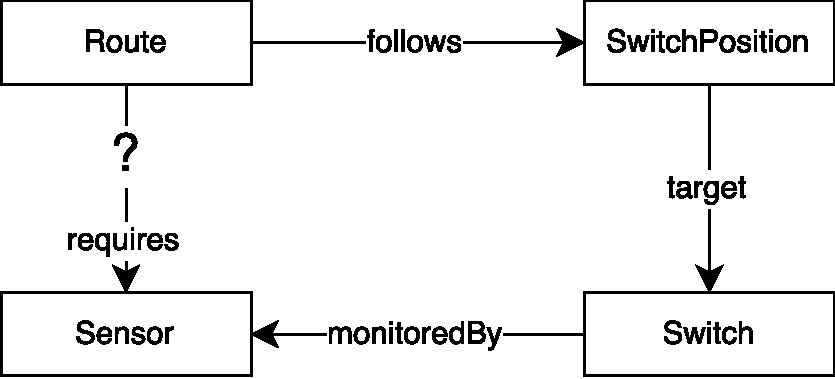
\includegraphics[width=0.7\linewidth, keepaspectratio]{figures/RouteSensor.pdf}
	\caption{A \emph{RouteSensor} kényszer}
	\label{fig:RouteSensor}
\end{figure}

\subsection{SwitchSet}

A \emph{SwitchSet} kényszer teljesülésének feltétele, hogy amikor egy út aktív és az elején található szemafor szabad jelzést ad, akkor az összes váltónak olyan állásban kell lennie, hogy a vonat az adott úton haladjon végig.

\begin{figure}[!ht]
	\centering
	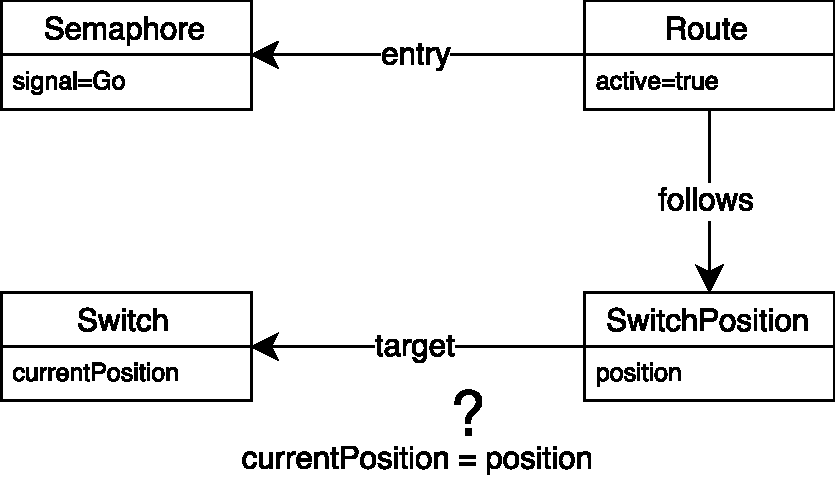
\includegraphics[width=0.7\linewidth, keepaspectratio]{figures/SwitchSet.pdf}
	\caption{A \emph{SwitchSet} kényszer}
	\label{fig:SwitchSet}
\end{figure}

?? valami még kéne

\section{A fejlesztés lépései}

A valóságban egy ilyen modell folyamatosan bővül, azáltal, hogy új sínpályákat építenek, felújítják a régieket, az állomásokat. Ezáltal a számítógépes modellt is bővíteni kell, ami programozók feladata. Ilyen esetben előfordulnak hibák, amiket javítani kell. Ennek a szimulálására a Train Benchmark 3 különböző szcenáriót különböztet meg: \emph{Batch}, \emph{Inject}, \emph{Repair}.

\subsection{\emph{Batch}}

Ebben az esetben azt szimulálja a Train Benchmark, hogy az adatbázisba betöltenek egy modellt és ellenőrzik a kényszereket. Ez a fejlesztés első szakasza. A tesztelés célja mérni, hogy milyen gyorsan lehet egy már kész modellt importálni és a kényszereket először, mindenféle háttértudás nélkül ellenőrizni.

\subsection{\emph{Inject}}

Az \emph{Inject} szakaszban véletlenszerű hibainjektálás történik a modellbe és minden ilyen után egy újraellenőrzés következik. Ezáltal lehet mérni, ha egy modellben kis változtatásokat hajtanak végre, akkor az adott adatbázis-kezelő ezt mennyire ismeri fel, ezáltal képes-e a modell kis részét megváltoztatni és esetleg csak ezt újraellenőrizni. A hibainjektálás a különböző kényszerekhez más és más módon zajlik. A \emph{RouteSensor} megsértéséhez egy úthoz tartozó véletlenszerű \emph{requires} élet törlünk, a \emph{SwitchSet} megsértéséhez pedig a megfelelő váltó \emph{currentPosition} tulajdonságát érvénytelen értékre állítjuk.

\subsection{\emph{Repair}}

Ebben a fázisban a hibák kijavításának szimulálása zajlik. Itt is a javítást követően a kényszerek ismételt ellenőrzése következik. A javításhoz a hibabeszúráshoz képest általában sokkal több erőforrásra van szükség, mivel itt először meg is kell keresni a hibát, és csak utána lehet kijavítani. Ezt a \emph{RouteSensor} esetében  a hiányzó \emph{requires} él pótlásával, a \emph{SwitchSet} esetében a váltó \emph{currentPosition}-jének a \emph{SwitchPosition} \emph{position}-jéhez való igazításával lehet megtenni.

\section{\emph{Tool}-ok}

A Train Benchmark 10 különböző \emph{Tool}-ra, azaz adatbázis-kezelő szoftverre készült el. Ezek között található a napjainkban legelterjedtebb relációs adatbázis-kezelő, \emph{Eclipse Modeling Framework}-öt használó, illetve \emph{RDF}-alapú és gráfadatbázis is. A dolgozat ezek közül az \emph{RDF}-alapú Jena és  RDF4J futtatását követelte meg, így ezeket emelném ki. Az \emph{RDF} egy egyszerű gráfmodell leíró nyelv adatok közlésére a világhálón. Nagy előnye, hogy akkor is összefűzhető két ilyen módon leírt modell, ha különböző sémára épülnek. Mindezt úgy teszi lehetővé, hogy adathármasokat (\emph{triple}) tárol, ami a következőkből épül fel:
\begin{itemize}
	\item \emph{subject}: Az adathármas alanya, rá vonatkozik a \emph{triple}-ben tárolt adat.
	\item \emph{predicate}: Tulajdonság, a \emph{subject} és az \emph{object} közötti kapcsolat típusát írja le.
	\item \emph{object}: A tulajdonság tárgya, leírhat egyszerű tulajdonságot is, de amennyiben a predicate két, a modellben szereplő elem kapcsolatának típusát jelöli, akkor egy másik modellbeli elemet fog jelenteni.
\end{itemize}

\emph{Subject}, \emph{predicate}, \emph{object} hármas lehet a következő: \emph{Magyarország}, \emph{tengerpart}, \emph{nincs}; míg lehet az is, hogy \emph{Magyarország}, \emph{szomszéd}, \emph{Ausztria}. Míg az első esetben a predicate egy tulajdonságot jelölt, a második esetben egy kapcsolatot egy másik hasonló elemmel.

Az \emph{RDF4J}-ben és a \emph{Jena}-ban az a közös, hogy mindkettő egy Java keretrendszer \emph{rdf} alapú adatok feldolgozására, lekérdezésére és módosítására. Mindkettő \emph{SPARQL} lekérdező nyelvet használ.
%----------------------------------------------------------------------------
\chapter{Gráfadatbázisok}
%----------------------------------------------------------------------------

Gráfadatbázisnak nevezünk minden olyan adatbázist, ahol az adat és/vagy a séma gráffal van reprezentálva, és minden adatmanipuláció egy gráftranszformációnak feleltethető meg. Sokféle implementáció terjedt el, ami illeszkedik erre a definícióra. Különbséget tehetünk az alapján hogy a csúcsokban csak egyedeket tárolunk vagy a csúcsok csak azonosítók és az éleken keresztül a leveleken vannak a tulajdonságaik. Másik megközelítés, hogy az éleknek lehetnek-e tulajdonságaik vagy nem, illetve irányított vagy nem irányított a kapcsolat. 

A struktúrájából adódóan olyan adatok leírására alkalmasak leginkább, ahol az egyedek közötti kapcsolat számottevő. Az éleken keresztül könnyen lehet navigálni, ezért alkalmasak közösségi hálózatok, keresőmotorok implementálására. 

\section{Példa gráfadatbázis használatára}

A gráfadatbázisok bemutatására a legáltalánosabb a közösségi hálózatok példája. Ennek alapja, hogy személyekről tárolunk bizonyos információkat, továbbá tároljuk a közöttük lévő kapcsolatokat. Esetünkben ez a kapcsolat legyen egyfajta és jelentse azt, hogy két ember ismeri egymást (barátok). Tároljuk a személyekről a következő adatokat:
\begin{itemize}
	\item Név
	\item Személyiigazolvány-szám
	\item További barátok listája
\end{itemize} 
Ezt egy relációs adatbázisban nehezen tudjuk megtenni, ugyanis a barátok listáját egy tömbben vagy lista típusban lenne célszerű tárolni, azonban a legtöbb relációsadatbázis-kezelő ezt nem támogatja. Általában egy második tábla felvételével szokták ezt megoldani. Ez a második tábla csak a kapcsolatok leírását szolgálja.

\begin{figure}[H]
	\centering
	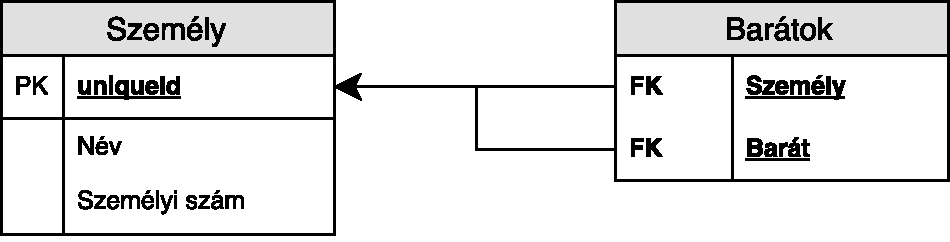
\includegraphics[width=100mm]{figures/RelaciosPelda.pdf}
	\caption{Példa relációs táblával való leírásra.}
	\label{fig:relaciosPelda}
\end{figure}

Amennyiben egy személy barátainak nevét szeretnénk megkapni, akkor ennek a relációs kalkulussal való kifejezése a következőképpen írható le:

\begin{equation}
\begin{split}
\{t^{(3)}\ | Szem\acute{e}ly(t) \wedge{} (\exists{}u)Bar\acute{a}tok(u) \wedge{} (\exists{}v)Szem\acute{e}ly(v) \wedge{} \\ v[1] = \textquoteright{}uniqueid\textquoteright{} \wedge{} 
t[1]=u[2] \wedge{}u[1]=v[1]      \}
\end{split}
\end{equation}

Már egy ilyen egyszerű kérdés megválaszolásához is három táblát kell összekapcsolni. Ez hatalmas erőforrást igényel, nem is beszélve arról, hogy mi a helyzet akkor, ha tranzitív lezártat szeretnénk számolni a baráti kapcsolat mentén. Ilyen esetben sokkal célravezetőbb az, ha egy gráfadatbázisban tároljuk az elemeket. A baráti kapcsolat általában kétirányú dolog, így a példánkban irányítatlan gráfon ábrázoljuk a kapcsolatot, de irányított gráffal is lehetne, ez esetben minden él helyére két él kellene.

\begin{figure}[H]
	\centering
	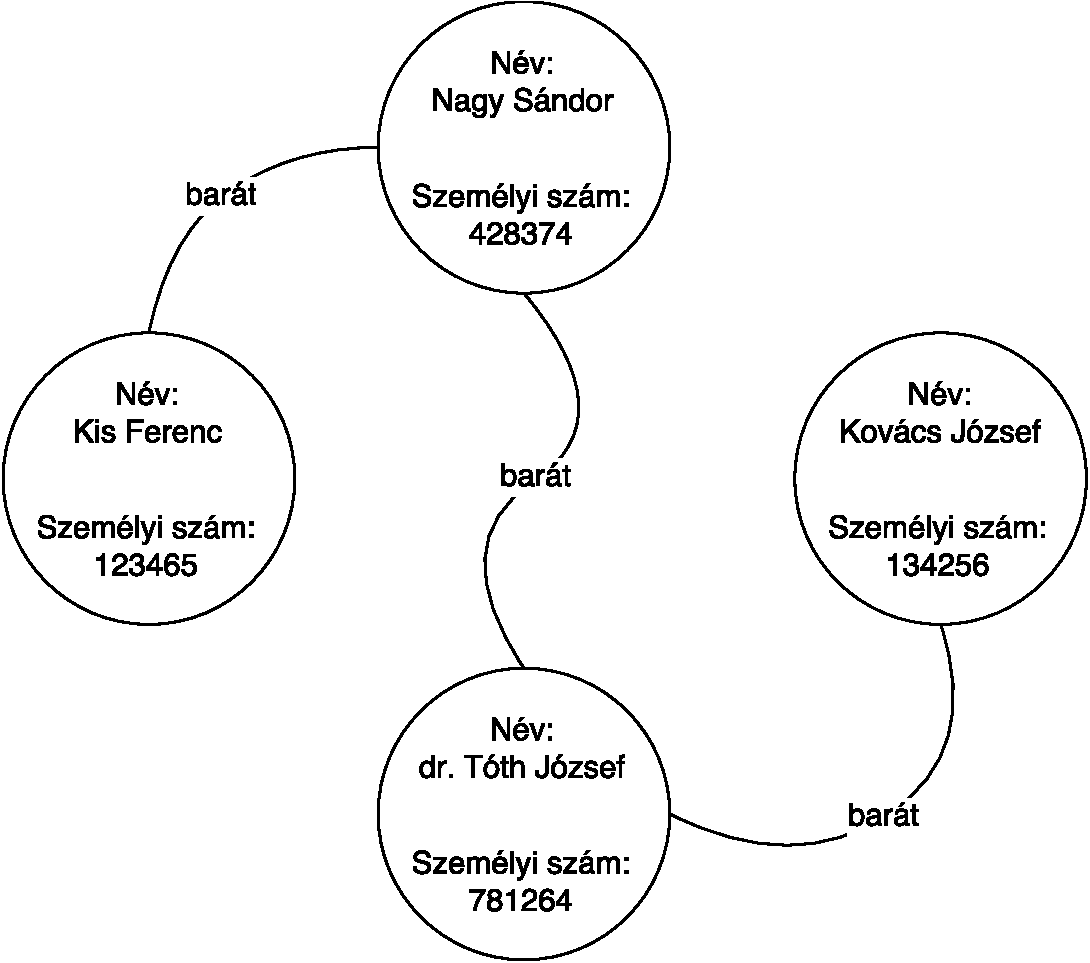
\includegraphics[width=100mm]{figures/GrafadatbazisPelda.pdf}
	\caption{Példa gráfadatbázisban való tárolásra.}
	\label{fig:grafPelda}
\end{figure}

A \ref{fig:grafPelda}. ábrán látható, hogy amennyiben valakinek barátait szeretnénk megtudni, a gráf élén végighaladva csak és kizárólag a barátainak az adatait fogjuk lekérni, senki másét nem. Ezáltal rengeteg memóriát és számolási időt takaríthatunk meg.
%----------------------------------------------------------------------------
\chapter{Graph Engine}
%----------------------------------------------------------------------------

A Graph Engine a Microsoft cég egyik projektje, amit 2010. október 30-án indítottak el, akkor még \emph{Trinity} néven. Ez egy gráfadatbázis-rendszer ami memóriafelhőn fut. A memóriafelhő egy globálisan címezhető, memóriában található kulcs-érték tároló. Mivel memóriaalapú, ezért gyors véletlen elérést biztosít nagyméretű gráfok esetén is, támogatja a gyors gráfbejárást és a párhuzamos feldolgozást is.

Az elkészített megoldás Microsoft Windows 7 x64 operációs rendszeren, Visual Studioban készült és \Csh{} nyelven, ezért a továbbiakban leírtak erre a környezetre vonatkoznak.


\section{A Graph Engine felépítése}

\section{\emph{TSL}}

A \emph{TSL}, azaz \emph{Trinity Specification Language} a Graph Engine gráfséma-leíró nyelve. Az előre definiált adatstruktúra helyett nagy könnyebbséget kínál azáltal, hogy szerveroldalon az adott alkalmazásra specifikus adatstruktúrát adhatunk meg. Szintaxisát tekintve leginkább a C, \cpp{}  és a \Csh{} nyelvre hasonlít.

A \emph{TSL} lehetőséget kínál sokfajta beépített típus használatára, melyek a következők:
\begin{itemize}
	\item \texttt{bool} \--- logikai
	\item \texttt{char} \--- karakter
	\item \texttt{int8, uint8, int16, uint16, int32, uint32, int64, uint64} \--- egész szám 
		
		Az \texttt{u} azt jelöli, hogy előjel nélküli, a szám pedig azt, hogy hány bites.
	\item \texttt{CellId} \--- 64 bites előjeles egész szám
		
		A különbség a \texttt{Cellid} és az \texttt{int64} között a programozó irányába hordozott jelentésben van. A \texttt{CellId}-t cellák egyedi azonosítójára való hivatkozásra használják.
	\item \texttt{float, double} \--- lebegőpontos szám
		A \texttt{float} 32, a \texttt{double} 64 bites.
	\item \texttt{decimal} \--- fix pontosságú szám 128 biten tárolva
	\item \texttt{DateTime} \--- dátum
	\item \texttt{Guid} \--- 128 bites egyedi azonosító
\end{itemize}

A Graph Engine egy ilyen \emph{TSL} fájl alapján építi fel az adatbázis sémáját. Ennek a fájlnak a kiterjesztési \emph{.tsl} és a következő elemekből épül fel:
\begin{itemize}
	\item \texttt{include \ldots{}} \--- Az \emph{include} után megadott fájlt ennek a fájlnak az elejére fűzi.
	\item \texttt{enum\{\ldots{} \}} \--- Felsorolás típust írhatunk le benne hasonlóan, mint C-ben.
	\item \texttt{struct structNeve \{\ldots{} \}} \--- Személyre szabható típus. Beépített típusok, konténerek és más \texttt{struct}-ok helyezhetőek el benne. A \emph{TSL} háromféle konténer típust támogat:
	\begin{itemize}
		\item \texttt{Array<T>} \--- T típusú elemek tömbje. Csak beépített típust támogat.
		\item \texttt{List<T>} \--- T típusú elemek listája. Előnye a tömbbel szemben, hogy dinamikus méretű elemek (konténerek) is tárolhatóak benne. A \Csh{}-ban lévő \texttt{List<T>}-nek megfeleltethető.
		 \item \texttt{string} \--- Karakterek sorozatát lehet benne tárolni.
	\end{itemize}
	\item \texttt{cell cellaNeve\{\ldots{} \}} \--- Struktúráját tekintve hasonló a \texttt{struct} típushoz, ellenben minden \texttt{cell}-hez tartozik egy egyedi azonosító (\texttt{CellId}), amin keresztül hivatkozni lehet rá. 
	\item Attribútumok \--- Stringek kulcs-érték párosa. Segítségükkel futási idejű információt lehet adni az adott celláról vagy mezőjéről.
	\item \texttt{protocol, server, proxy} \--- Távoli adatbázis-elérést lehet velük konfigurálni.
\end{itemize}

A \emph{TSL}-t külön projektbe kell elhelyezni. Fordítása után egy \emph{dll} könyvtár jön létre, amit a másik \Csh{} projektünkhöz hozzálinkelhetünk. Amennyiben a Graph Engine beépített projektjét használjuk és egy \emph{solution} alatt dolgozunk, akkor ezt a Visual Studio elvégzi helyettünk. 

\subsection{Példa \emph{TSL} fájlra}

A példában egy baráti társaságban lévő emberekről tárolunk adatokat. Ezek az adatok legyenek a következők minden embernél: név, személyiigazolvány-szám, barátok. Sokféle megoldás létezhet ennek a problémának a leírására, mivel a nevet tárolhatjuk egy \texttt{string}-ben, de akár egy struktúrában is, a személyiigazolvány-szám lehet fix hosszúságú 6 karakter vagy lehet egy változó hosszú \texttt{string}. Esetünkben a név egy struktúra, a  személyiigazolvány-szám pedig \texttt{string} típusú.

\begin{figure}[ht!]
	\centering
	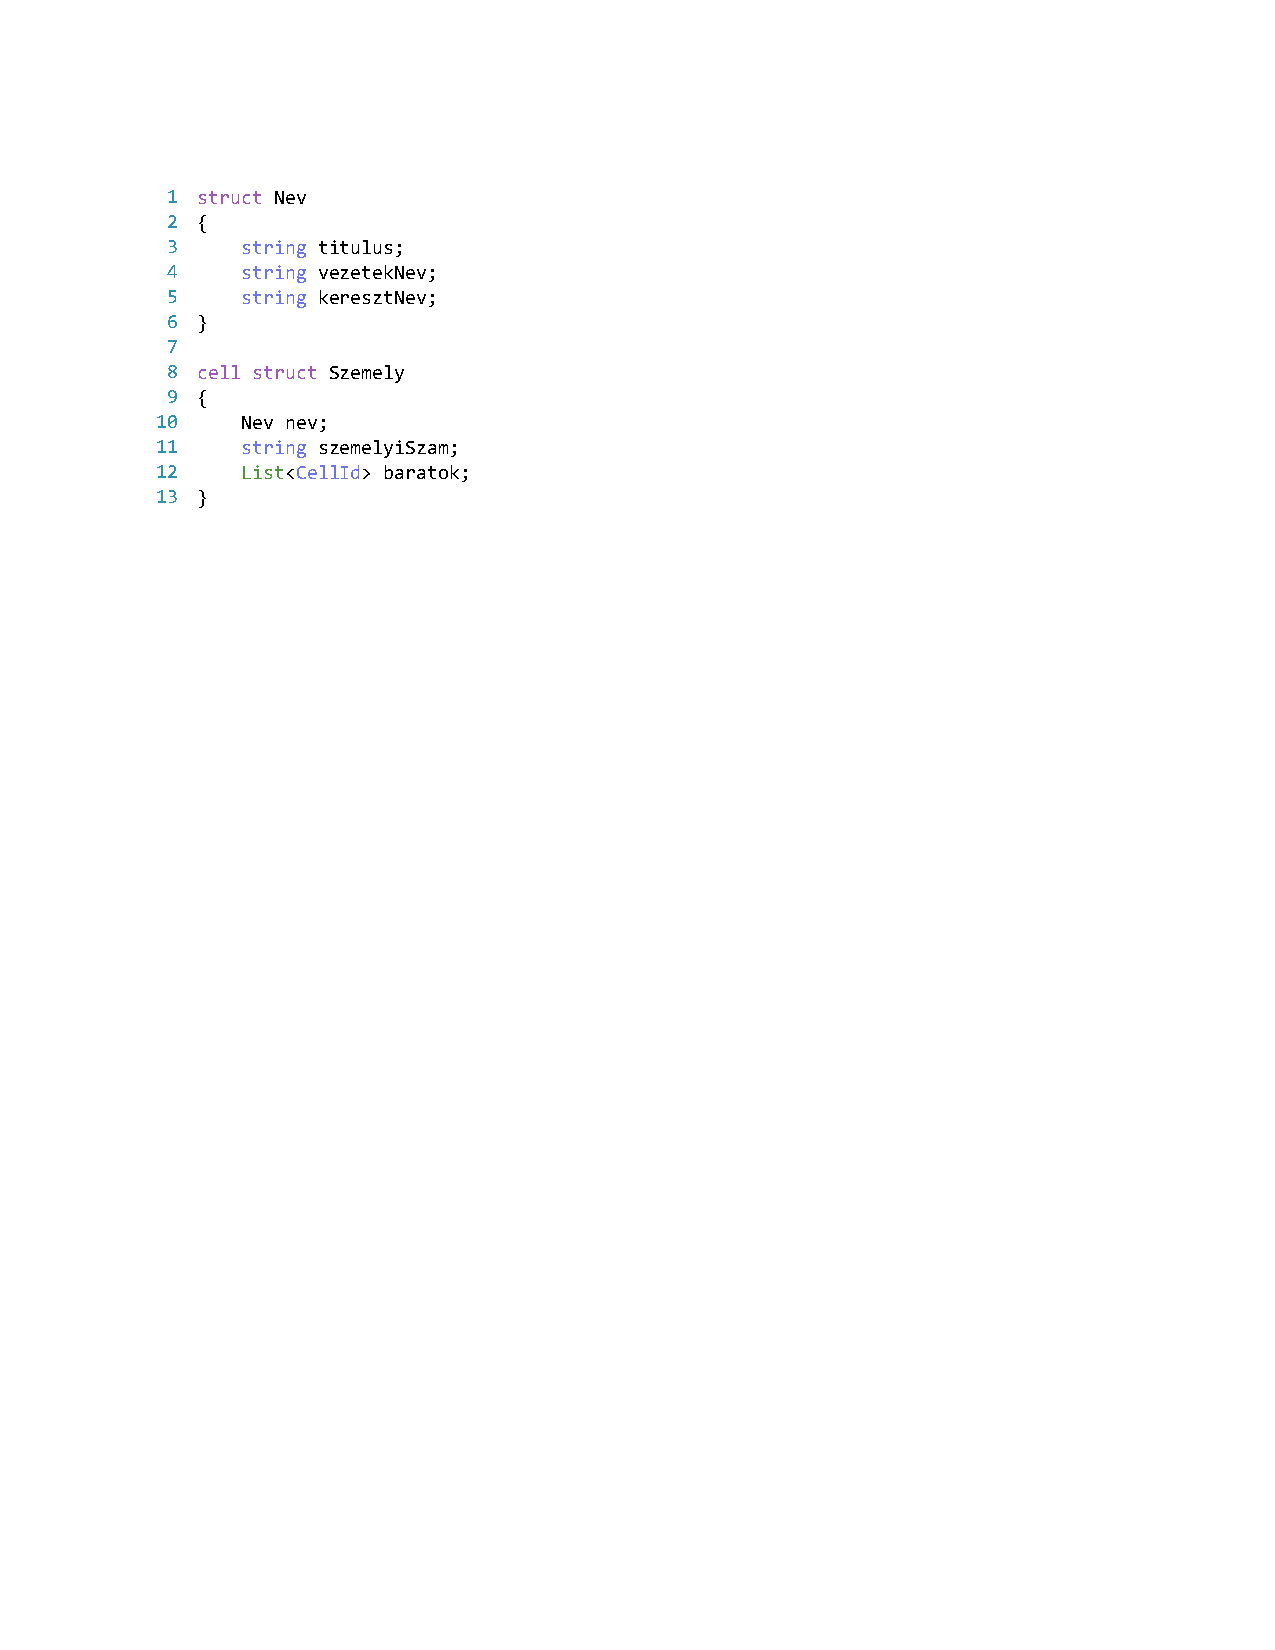
\includegraphics[]{figures/TarsasagTSL.pdf}
	\caption{Példa TSL használatára.}
	\label{fig:TSL}
\end{figure}

\section{Adatelérés}

A Graph Engine a \texttt{cell} típushoz készít úgynevezett \emph{Accessor}-okat, melyek az adatolvasást és manipulálást könnyítik meg. Ezzel párhuzamosan létrehoz osztályokat, amiket a Visual Studioban lévő IntelliSense is tud kezelni, megkönnyítve a további implementációs munkát. Az \emph{Accessor}-ok használatát is a fenti példán keresztül mutatnánk be. Fordítás után a következő metódusokat tudjuk használni: 
\begin{itemize}
	\item \texttt{Global.LocalStorage.IsSzemely(long cellId)} \--- A \emph{cellId} azonosítójú elemről megállapítja, hogy Szemely típusú-e. Visszatérési értéke: \texttt{bool}.
	\item \texttt{Global.LocalStorage.LoadSzemely(long cellId)} \--- Visszatérési értéke egy Szemely típusú objektum, aminek a CellId-je a függvény bemeneteként megadott paraméter.
	\item \texttt{Global.LocalStorage.SaveSzemely(\ldots{})} \--- A függvény bemeneti paraméterének megadott adatok alapján elment egy személyt az adatbázisba. Ez a paraméter lehet Szemely típusú objektum, de megadhatjuk felsorolva az osztály mezőit (\texttt{cellId, nev, szemelyiSzam, baratok}) is. Amennyiben létezik az adott \texttt{cellId}-vel rendelkező bejegyzés, akkor felülírja.
	\item \texttt{Global.LocalStorage.Szemely\_Selector()} \--- Visszatérési értéke egy IEnumerable<Szemely> lista, amiben az adatbázisban szereplő összes személy benne van. Végigiterálva ezen a listán, megkaphatjuk a személyek adatait.
	\item \texttt{Global.LocalStorage.Szemely\_Accessor\_Selector()} \--- Hasonló a texttt{Szemely\_Selector}-hoz, ellenben IEnumerable<SzemelyAccessor>-ral tér vissza, azaz nem személy osztályú elemekkel, hanem azok \emph{Accessor}-aival.
	\item \texttt{Global.LocalStorage.UseSzemely(long cellId)} \--- Az adott \emph{cellId}-vel rendelkező személy \emph{Accessor}-át adja vissza. Ezen keresztül tudjuk módosítani a bejegyzést. Használat után mindenképp fel kell szabadítani, ezért \emph{using} blokkba érdemes illeszteni.
\end{itemize}

Sajnálatos módon a Graph Engine egyelőre nem támogatja az egymásba ágyazott \emph{Accessor}-ok használatát. Emiatt ha például amennyiben két ember adatait szeretnénk összehasonlítani, akkor először az egyik, majd a másik adatait kell kimentenünk a lokális memóriába, majd összehasonlítani. Erre a problémára megoldást nyújthat a \emph{Language-Integrated Query (LINQ)}, illetve \emph{Language Integrated Knowledge Query (LIKQ)} használata, melyek lehetőséget kínálnak lekérdezések írására.

\subsection{\emph{LINQ}}

A \emph{Language-Integrated Query}, azaz \emph{LINQ} a .NET 3.5 óta létező szolgáltatás, ami megkönnyíti az adatelérést a programozó számára. Célja a nem, vagy csak részben objektum-orientált adatforrások általános célú feldolgozása. Kezdetben az \emph{SQL}- és az \emph{XML} nyelvet támogatta, mivel a relációs adatbázisok és az XML fájlok a két legelterjedtebb, nem objektum-orientált adatforrás.

\begin{figure}[H]
	\centering
	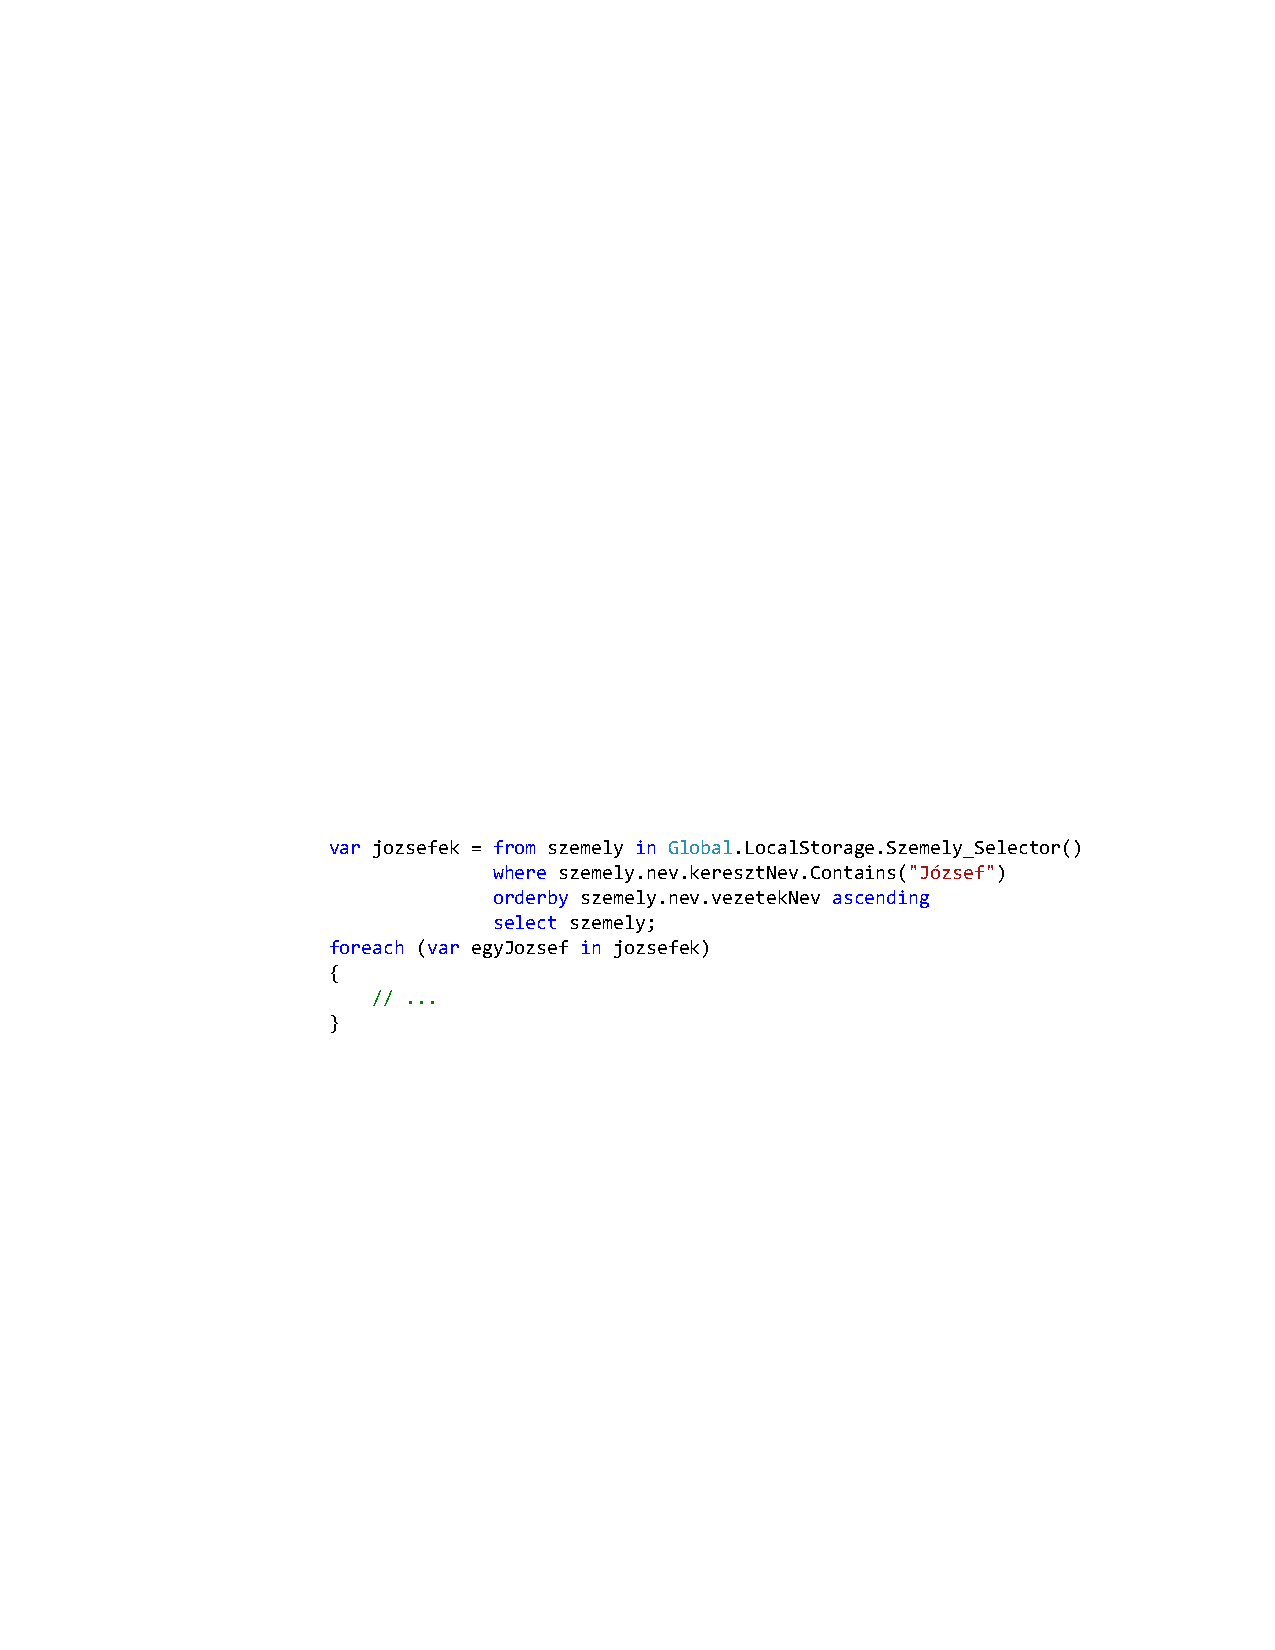
\includegraphics[]{figures/JozsefekLINQ.pdf}
	\caption{Egy egyszerű LINQ lekérdezés. A József keresztnevű emberek adatait lehet kinyerni így.}
	\label{fig:LINQ}
\end{figure}

Egy \emph{LINQ} lekérdezés felépítése hasonló az \emph{SQL} nyelv szintaxisához. A \emph{from, where, orderby, select} kulcsszavaknak a jelentése megegyezik. Legfőbb különbség azonban, hogy míg az \emph{SQL}-nél először azt kell megadni, hogy mit szeretnénk, aztán pedig, hogy honnan, addig a \emph{LINQ}-nél ez fordítva van. Ez nagy előny, mivel így az \emph{IntelliSense} már felajánlja az adott osztály mezőit, függvényeit kiegészítésként, emellett fordítás előtt ellenőrizni lehet az esetleges elgépeléseket. A \emph{select} után megadhatunk \emph{property}-ket, anonym-osztályt, de akár, ahogy a \refstruc{fig:LINQ} mutatja, a teljes osztályt is.



\subsection{\emph{LIKQ}}



\section{Példaalkalmazás}
%----------------------------------------------------------------------------
\chapter{Implementáció}
%----------------------------------------------------------------------------

Az elkészült program \emph{Visual Studioban} egy \emph{solutionből}, azon belül két projektből áll. Az egyik projekt a \emph{TSL} fájlt tartalmazza, ez felel az adatbázis felépítéséért, a másik pedig a \Csh{} forrásfájlokat, ez az adatbázis szempontjából a kliensoldalt valósítja meg. A fejlesztést nagyban megkönnyítette, hogy ilyen esetben egyetlen kattintással tudjuk fordítani a két projektet. A továbbiakban először a \emph{TSL} projekt, majd a \emph{Trainbenchmark} nevű \Csh{} fájlokat tartalmazó projekt kerül bemutatásra.

\section{\emph{TrainBenchmarkTSLProject}}

A projekt egyetlen \emph{.tsl} kiterjesztésű fájlból áll. Ez tartalmazza a Train Benchmark modelljének a Graph Engine-ben megfelelő leírását néhány módosítással. A modellben két osztály közötti kapcsolat a gráfban lévő éleket határozzák meg. Az osztályok a gráf csúcsai lesznek. A \emph{TSL} nem támogatja az öröklést, így azokhoz az osztályokhoz, amik öröklődnek fel van véve a szülő összes tulajdonsága. Ez a \emph{Segment} és a \emph{Switch} esetében lényeges, amik a \emph{TrackElement} osztályból öröklődnek, ezért mindkettő tartalmaz \emph{connectsTo} listát.

A Graph Engine-ben a kapcsolatok nem típusfüggőek, minden gráfél \emph{CellId} típussal mutat egy cellára. Ez nagy könnyedség, hiszen amennyiben nem így lenne, azaz meg kéne határozni, hogy egy él milyen osztályú cellára mutat, akkor a \emph{TrackElement} \emph{connectsTo} éleit nem lehetne megvalósítani, ugyanis egy \emph{Segment} élen keresztül csatlakozhat \emph{Switch}-hez és egy másik \emph{Segment}-hez is.

A módosított modell a \ref{fig:GraphEngineTSLModel} ábrán látható. A különbségek, amik ez a modell és a Train Benchmark eredeti modellje között van, az csak az öröklés miatti \emph{connectsTo} élekben van, így a két modell matematikai szempontból ekvivalens.

Az éleknek két fajtája van. Sima \emph{CellId} típusú élek egy-egy kapcsolatot jelölnek, míg a \texttt{List<CellId>} egy-több kapcsolat leírására szolgál. Ez azt jelenti, hogy egy csúcsból egy éltípussal egy másik típusú csúcsba egy él vezet vagy vezethet több másik típusú csúcsba is egy-egy él.

A \texttt{Position}, illetve \texttt{Signal} felsorolásokat is a \emph{TSL} fájlban érdemes leírni, így a gráf csúcsaiban már tárolva vannak.

\begin{figure}[H]
	\centering
	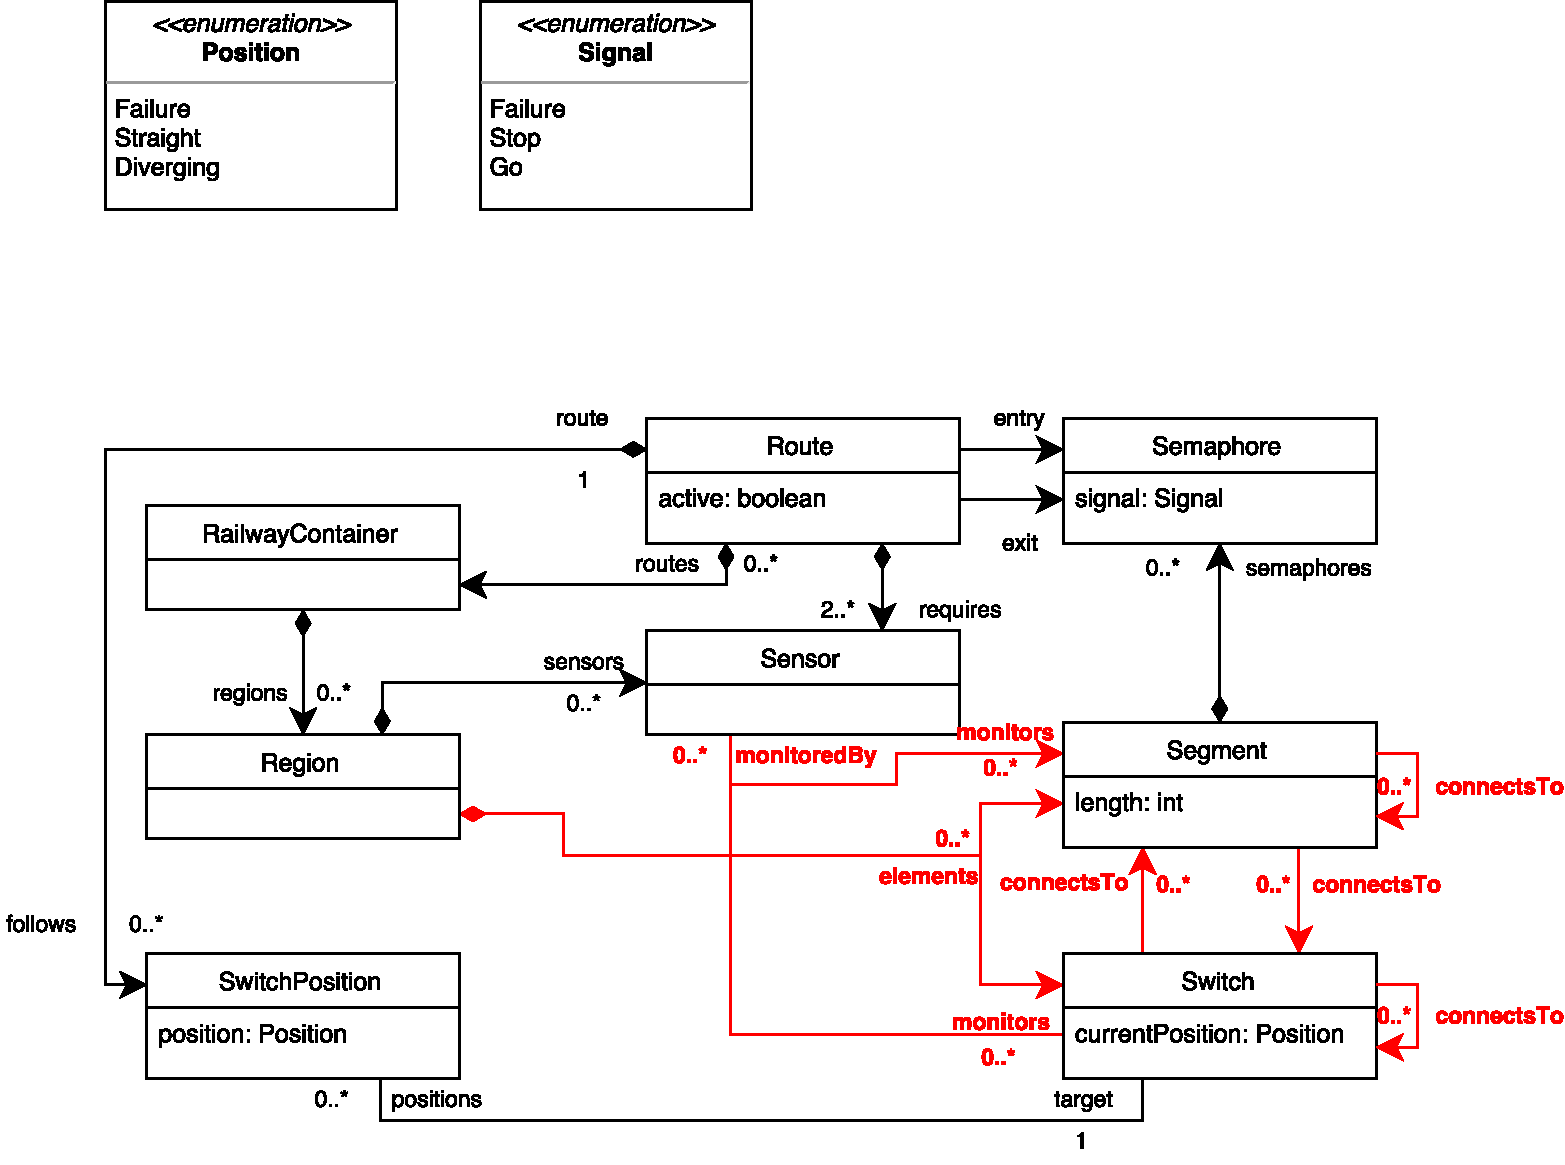
\includegraphics[width=\linewidth, keepaspectratio]{figures/GraphEngineTSLModel.pdf}
	\caption{A \emph{TSL} modell felépítése.}
	\label{fig:GraphEngineTSLModel}
\end{figure}

\section{\emph{\Csh{} project}}

A projekt 7 forrásfájlból és 41 függőségből (\emph{Reference}) épül fel. A függőségek között megtalálható a \emph{TSL} projekt. A Graph Engine használata egy projekten belül globális, így minden osztály és függvény ugyanazokon az adatokon dolgozik.

\subsection{A program belépési pontja}

A \texttt{Program.cs}-ben megtalálható \texttt{Main} függvény a program belépési pontja. Ebben található néhány alapvető konfiguráció, melyeknek két fő célja van.
\begin{itemize}
	\item A futási idő méréséhez a futtató folyamatot a 2-es processzormagon van futtatva, mert a háttérben futó folyamatok és szolgáltatások jelentős része az 1-es számú processzormagot használja. Így nagyobb eséllyel fut a program tisztább környezetben.
	\item A Graph Engine motorja lokális futásra van konfigurálva, ezáltal nem használ hálózati erőforrást, nincs a lekérdezéseknek felesleges \emph{overhead}-je.
\end{itemize}

Itt található még egy iteráció, mely végigmegy az előre elkészített modelleken méret szerint, és mindegyik méretre végrehajtatja a mérést. A mérés lépései a \texttt{Test.cs} fájlban találhatóak. Minden mérés három lépésből (beolvasás, validáció, módosítás) áll. Egy lépésben a program végrehajtja a modellen a megfelelő műveletet, és az ezalatt eltelt időt tároljuk el.

\subsection{Beolvasás}

A beolvasás a modell \emph{.ttl} fájlból való feldolgozását, majd az adatbázisba való mentését jelenti. Az \emph{RDFReader} osztály \texttt{read()} metódusa valósítja meg. A \emph{.ttl} fájl \emph{Turtle} formátumot takar. Ez egy olyan fájltípus, mely alkalmas az \emph{RDF} típusú gráfok tárolására. 

Több olyan könyvtár létezik a .Net-hez, ami \emph{Turtle} típusú fájlokat tud feldolgozni. Ezek közül a \emph{dotNetRDF} nevű ingyenes és nyílt forráskódú könyvtárat használja a program. Ennek kezelése egyszerű, jól átlátható. A \emph{Turtle} állományban található \emph{Triple}-öket beolvassa a memóriába és készít egy gráfot, amit már gyorsan be lehet járni. Az elkészült gráf bejárása a következőképpen zajlik:

\begin{itemize}
	\item Kiválasztjuk egy listába azokat a \emph{Triple}-öket, melyek a csúcsok típusát írják le.
	\item Végigiterálunk a listán és minden csúcshoz létrehozunk egy megfelelő típusú osztályt.
	\item Megkeressük azokat a további \emph{Triple}-öket, melyek az adott csúcshoz tartoznak és a hozzá kapcsolódó tulajdonságokat, éleket tárolják, majd ezeket az információkat beleírjuk az osztályunkba.
	\item Az elkészült osztályt elmentjük a Graph Engine adatbázisába.
\end{itemize}

A feldolgozás folyamán két konverzióra van szükség, mégpedig azért, mert a \emph{Turtle} fájlban egyszerű szövegként van tárolva a \emph{Signal} és a \emph{Position}. Ezeket \emph{enum}-má kell konvertálni, hogy a Graph Engine csúcsaiba tulajdonságként el tudjuk menteni.

\subsection{Validáció}

Ebben a lépésben a modell ellenőrzése következik. Mindkét kényszer esetén fontos az is, hogy a modellben hol sérülnek, mivel egy valós fejlesztési folyamat során is fontos, hogy a tervező ki tudja javítani a problémákat és ezt csak úgy tudja megtenni, ha tudja, hogy hol vannak. Így egyik esetben sem elég megtalálni az első olyan pontot a modellben, ahol a kényszer nem teljesül. Ez a programban úgy lett megvalósítva, hogy bejárja az egész modellt és összeszámolja a hibás helyeket.

A modellvalidációs osztály a \emph{Validator} nevet viseli. Két függvényből áll, melyek a \texttt{SwitchSet()} és a \texttt{RouteSensor()}, a két megvalósított kényszer neve alapján. Mindkét függvény egy egész számot ad eredményül, ami azon elemek számát jelöli, melyek nem felelnek meg a követelményeknek. 

\subsubsection{\emph{SwitchSet}}

A \emph{SwitchSet} kényszer ellenőrzéséhez az összes modellben szereplő \emph{Route}-on, melynek kezdetén a \emph{Semaphore} \emph{Signal}-ja \emph{Go} értékű, lévő \emph{SwitchPosition} és a hozzátartozó \emph{Switch} \emph{Position} tulajdonsága meg kell egyezzen. Ezért a függvényben először a \emph{Semaphore}-okon iterálunk végig, majd azokon az utakon, melyeknek kezdőpontja az adott \emph{Semaphore}, végül pedig a hozzá tartozó \emph{SwitchPosition} és az ahhoz tartozó \emph{Switch} tulajdonságait kérjük le. A folyamat forráskódja a ábrán látható.
%TODO ábra

Több típusú csúcson kell műveleteket végezni, ezáltal a \emph{LINQ}-es lekérdezések eredményét használat előtt el kell tárolni egy lokális változóban a \texttt{ToList()} függvény segítségével. Enélkül a \ref{graphenginelinq} fejezetben tárgyalt okok miatt holtpont alakulna ki. Az egymás utáni \texttt{using} blokkok használatánál is ugyanilyen módszerrel el kell tárolnunk az adott változó értékét.

\subsection{Módosítás és újraellenőrzés}

A modellen történő módosításokat a \emph{Modifier} osztály végzi. Négy különböző eset van, az alapján, hogy a \emph{SwitchSet} vagy a \emph{RouteSensor} kényszer kapcsán történik a módosítás, illetve \emph{Inject} vagy \emph{Repair} a célja. A modell elrontása egyszerűbb művelet a javításnál, ugyanis nem kell hibát keresni és azt kijavítani, elég csak megkeresni egy elemet és a megfelelő értékét hibásra állítani. Ezt követi az újraellenőrzés, ami a validációs szakasz ismételt futtatását jelenti. A módosítás és az újraellenőrzés ilyen sorrendben egymás után többször végrehajtódik.

\subsection{Mérés és az eredmények elmentése}

Minden szakasz futási ideje a \emph{System.Diagnostic.StopWatch} osztály segítségével lett lemérve. A Train Benchmark többi \emph{Tool}-ja $ns$-ban ad eredményt a futás idejéről, azonban két azonos konfigurációjú , egymás után történő futtatás eredménye is legalább 100 $\mu{}s$-mal eltér. Ezen megfontolás miatt az elkészült program futásidő-mérésének pontossága 1 $\mu{}$s. A \emph{StopWatch} osztályban az \texttt{ElapsedTicks} és a \texttt{Frequency} \emph{property}-k segítségével lehet $ms$-nál pontosabb eredményt elérni. 

\section{Többi \emph{Tool} futtatása}

%----------------------------------------------------------------------------
\chapter{Mérési eredmények}
%----------------------------------------------------------------------------

Ebben a fejezetben a teljesítménymérések eredményének elemzéséről és a leszűrhető konklúziókról lesz szó. Összehasonlítjuk a Graph Engine teljesítményét a másik két eszköz teljesítményével. Kielemezzük a lehetséges okait a futási idők közötti különbségeknek.

\section{Mérés és az eredmények elmentése}

Minden szakasz futási ideje a \emph{System.Diagnostic.StopWatch} osztály segítségével lett lemérve. A többi Train Benchmark implementáció $ns$-ban ad eredményt a futás idejéről, azonban két azonos konfigurációjú , egymás után történő futtatás eredménye is legalább 100 $\mu{}s$-mal eltér. Ezen megfontolás miatt az elkészült program futásidő-mérésének pontossága 1 $\mu{}$s. A \emph{StopWatch} osztályban az \texttt{ElapsedTicks} és a \texttt{Frequency} \emph{property}-k segítségével lehet $ms$-nál pontosabb eredményt elérni.

A méréseket ötször egymás után hajtja végre a program és az eredményt egy \emph{csv} fájlba fűzi bele. Az öt egymás utáni futtatás nagyobb valószínűséggel ad konzisztens eredményt. A \emph{csv} minden sorába egy adott futtatás szakaszának (beolvasás, ellenőrzés, módosítás vagy újraellenőrzés) az eredménye kerül. A felépítése az alábbi oszlopokból áll:

\begin{itemize}
	\item \emph{Tool}: Annak az adatbázis-rendszernek a neve, amin a programot futtatjuk.
	\item \emph{Workload}: \emph{Inject} vagy \emph{Repair} lehet, az alapján hogy milyen teljesítményt mérünk, a hibainjektálást vagy a javítást.
	\item \emph{Description}: Leírást illeszthetünk ide. Ez az elkészült szoftver futtatása után üres lesz.
	\item \emph{Model}: A modell neve és mérete kerül ide.
	\item \emph{Run}: Aktuális futtatás sorszáma 1-től indexelve.
	\item \emph{Phase}: A futtatott szakasz típusa kerül ide, értéke \emph{Read}, \emph{Check}, \emph{Transformation} vagy \emph{Recheck} lehet.
	\item \emph{Iteration}: A módosítás és újraellenőrzés szakasz többszörös futtatásának sorszáma. A beolvasás- és a validációs szakaszban nincsen értéke.
	\item \emph{Time}: Az adott szakasz futtatása alatt eltelt idő $ns$-ban. Nem a teljesítménymérés kezdete óta eltelt időt jelzi.
\end{itemize}

A gép konfigurációja, melyen a méréseket végeztük a \ref{tab:System} táblázatban található. A meghajtón több, mint 20 GB szabad hely volt elérhető.

\begin{table}[H]
	\centering
	\begin{TAB}(r,20pt,20pt){|c|c|}{|c|c|c|c|c|} 
		Alaplap & Gigabyte Z87M-D3H \\
		Processzor & Intel\textregistered{} Core\texttrademark{} i5-4690K CPU @ 3.50GHz \\ 
		Memória & Kingston 8GB 1600MHz DDR3 Non-ECC CL11 \\
		Meghajtó & Kingston HyperX 3K 240 GB SSD  \\
		Operációs rendszer & Windows 7 Ultimate x64 Service Pack 1  \\ 
	\end{TAB}
	\caption{A gép konfigurációja}
	\label{tab:System}
\end{table}

Az elkészült program és a Train Benchmark többi teljesítménymérésének futtatása sok órás művelet. A modellek (amiken a teszteket végeztük) elemeinek a száma körülbelül 5 ezertől 9,3 millióig terjed kettes alapú logaritmikus skálán. Olyan esetben, amikor egy eszköz egy szakaszban lévő futási ideje túllépne egy bizonyos észszerű határt, akkor leállítjuk a teljesítménymérést. Ezt a határt a \emph{RouteSensor} esetében 100000 $ms$-nál, a \emph{SwitchSet} kényszer esetében 200000 $ms$-nál húztuk meg. Amennyiben bármelyik szakaszban (beolvasás, ellenőrzés vagy módosítás) a futási idő meghaladja ezt a határt, akkor értelemszerűen a többi szakaszban sem kapunk eredményt.

A tesztek eredményét a következő részeken keresztül mutatjuk be. Az első két példa a modell beolvasása után a \emph{RouteSensor} kényszer teljesülését ellenőrzi, majd az ahhoz kapcsolódó \emph{Inject}, illetve \emph{Repair} transzformációt hajtja végre. A második két példa a \emph{SwitchSet} kényszert követeli meg. Minden esetben, a modelleken ötször futtattuk le a teljes ciklust és azon belül a módosítás, újraellenőrzés fázisokat tizenháromszor, végül pedig az egész átlagából számoltuk ki az idő értékeket.

Minden eszköz tesztjét egy parancssori ablakból futtattuk, ezáltal törekedve arra, hogy más programok ne használják a számítógép erőforrásait. A tesztek után az eredmények kiértékelése céljából lefuttattuk úgy is, hogy közben a \emph{Visual Studio} beépített teljesítményanalízisével mértük, hogy melyik függvény végrehajtása tart a legtovább.

\section{A \emph{RouteSensor}-hoz tartozó \emph{Inject} eredményeinek értékelése}

A \ref{fig:RouteSensorInjectResult} ábra mutatja 6 diagramon a tesztelés eredményét. A diagramokon a függőleges tengely a futási idő $ms$-ban mért logaritmikus skáláját, míg a vízszintes tengely a modellek méretének skáláját mutatja. Ez utóbbi is logaritmikus skála, mert egy osztás alatt a modellek mérete duplájára növekszik. A diagramok tetején található felirat az adott futtatási fázist mutatják.

A továbbiakban egyesével a diagramokon látható eredményeket elemezzük. Az átláthatóság érdekében a vízszintesen egymás mellett elhelyezkedő diagramok skálája megegyezik.

\subsubsection{Read}

A \emph{Read} szakaszban a Graph Engine minden modell esetében az adatok beolvasása és feldolgozása több ideig tartott. Ennek oka az, hogy az \emph{RDF} formátum feldolgozását és memóriába másolását a használt könyvtár (\emph{dotNetRDF}) időigényesen végezte.

\subsubsection{Check}

A validációs szakasz során a kapott eredmények alapján a Graph Engine futási idejét lényegesen nem befolyásolta a modell mérete. Ennek valószínűsíthető oka, hogy az adatbázis felé indított kérés feldolgozási ideje lassú, de a kérést már gyorsan dolgozza fel, az adatok mennyiségétől függetlenül.

\subsubsection{Read and Check}

A \emph{Read and Check} diagram az előző kettő összegét mutatja. A beolvasási szakasz több nagyságrenddel nagyobb a validációsnál, így az a meghatározó. A Graph Engine hiába gyorsabb nagy modelleknél a validációs szakaszban, ez az előny az összesített időknél eltűnik. 

\pagebreak
\begin{figure}[H]
	\centering
	\vspace*{-2cm}
	\makebox[\linewidth]{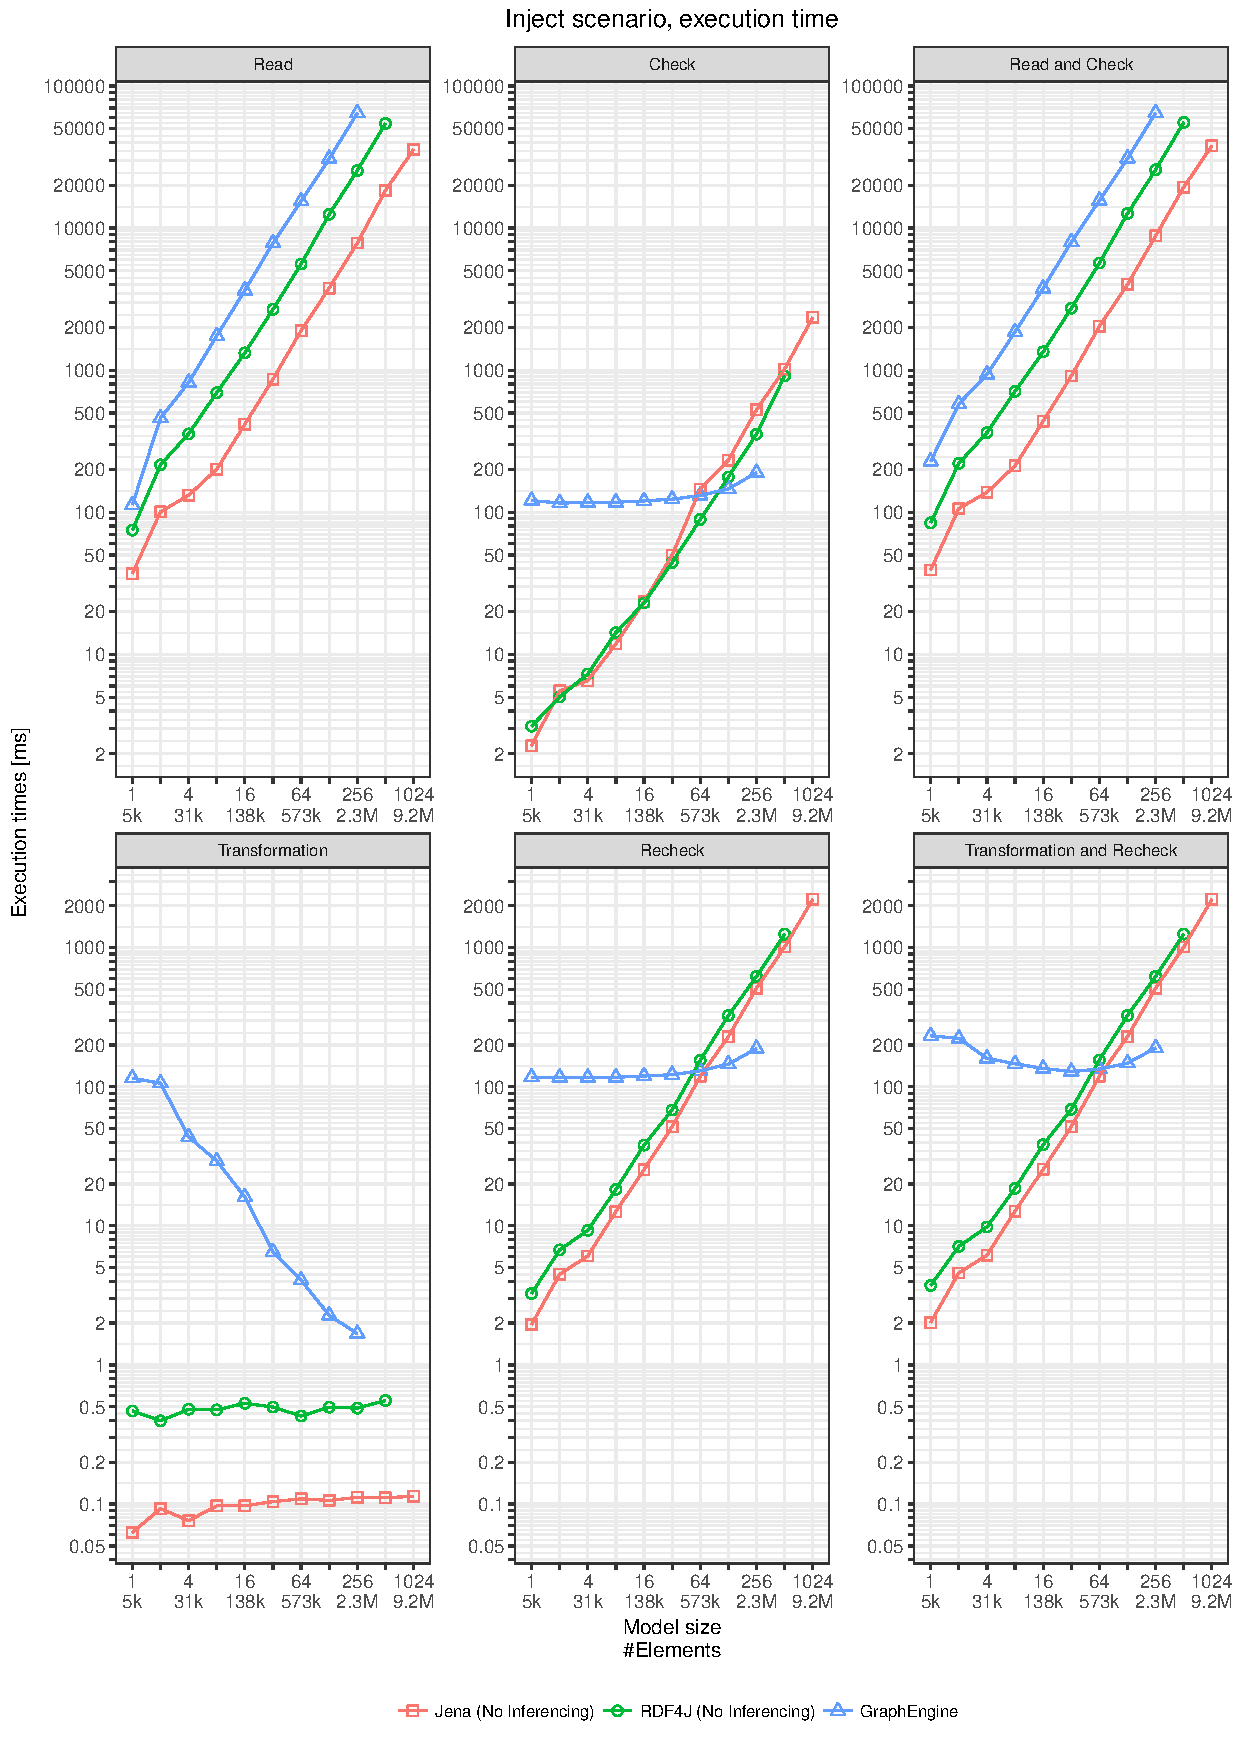
\includegraphics[width=1\linewidth]{figures/RouteSensor-times-Inject.pdf}}
	\caption{A hibainjektálás tesztelésének futási idejeinek eredménye a \emph{RouteSensor} esetében.}
	\label{fig:RouteSensorInjectResult}
\end{figure}

\subsubsection{Transformation}

A hibainjektálás során előre nem várt eredményt kaptunk. A modell növekedésével a Graph Engine teljesítménye nőtt, a futási idő rövidebb lett. Ennek oka, hogy kisméretű modelleken több lekérdezés kellett, hogy találjon olyan \emph{requires} élt, amit el lehet távolítani. Az \emph{RDF4J} és a \emph{Jena} esetében a modell mérete nem befolyásolta az eredményt. A \emph{Read} szakasz lassú futása miatt a legnagyobb méretű modelleken nem volt tesztelhető, hogy meddig csökkenne tovább.

\subsubsection{Recheck}

A \emph{Recheck} fázisban a \emph{Check} szakasszal megegyező eredményt kaptunk az összes eszköznél. Ennek oka, hogy nem tárolunk információt arról, hogy az előző validációs fázisban milyen eredményre jutottunk, ezáltal az újraellenőrzésnél ismét a teljes modellt be kell járni. Gyorsítható lenne a folyamat, ha eltárolnánk, hogy az előző ellenőrzés hol talált olyan csúcsokat, melyek nem feleltek meg a kényszernek és az újraellenőrzésnél a modell többi részében keresne csak hibákat. Azonban ehhez feltételezni kell, hogy ismerjük a szimuláció működését, azaz a transzformációs fázisban nem javítunk ki hibákat.

\subsubsection{Transformation and Recheck}

Hasonlóan a \emph{Read and Check} diagramon látható eredményhez, itt is az egyik fázis sokkal több idő alatt fut le, ezáltal az együttes eredményben dominál. Itt azonban a validációs fázis a meghatározó. Kis modellek esetén ugyan befolyásolja a Graph Engine eredményét, de nagyobb méretű modelleken nem.

\section{A \emph{RouteSensor}-hoz tartozó \emph{Repair} eredményeinek értékelése}

A \emph{Repair} tesztelés esetében a beolvasás és a validáció ugyanolyan eredményt adott, mint az \emph{Inject} esetében. Ez a várt eredmény, hiszen ugyanazok a függvények futottak le. Így csak a módosítás fázisban van eltérés.

A \ref{fig:RouteSensorRepairResultTransformation} ábrán a \emph{Transformation} és a \emph{Transformation and Recheck} fázisok futásidejei találhatóak. A várakozásnak megfelelően a Graph Engine módosítás fázisban töltött ideje a tesztelt modellekre nem csökkent, de nem is nőtt számottevően. A másik két eszköz esetében exponenciálisan növekedett a végrehajtási idő. Az \emph{RDF4J} és a \emph{Jena} esetében nem csak az \emph{Inject}, de a \emph{Repair} módosításnál is a modell ellenőrzése minden mért eredménynél több, mint tízszer annyi, így a \emph{Transformation and Recheck} szakasz idejét a \emph{Transformation} csak kis mértékben befolyásolja. Ezzel szemben a Graph Engine esetében a módosítás és az újraellenőrzés fázisok időben nagyságrendileg megegyeznek, így a kettő egyforma mértékben befolyásolja az eredményt.

\begin{figure}[H]
	\centering
	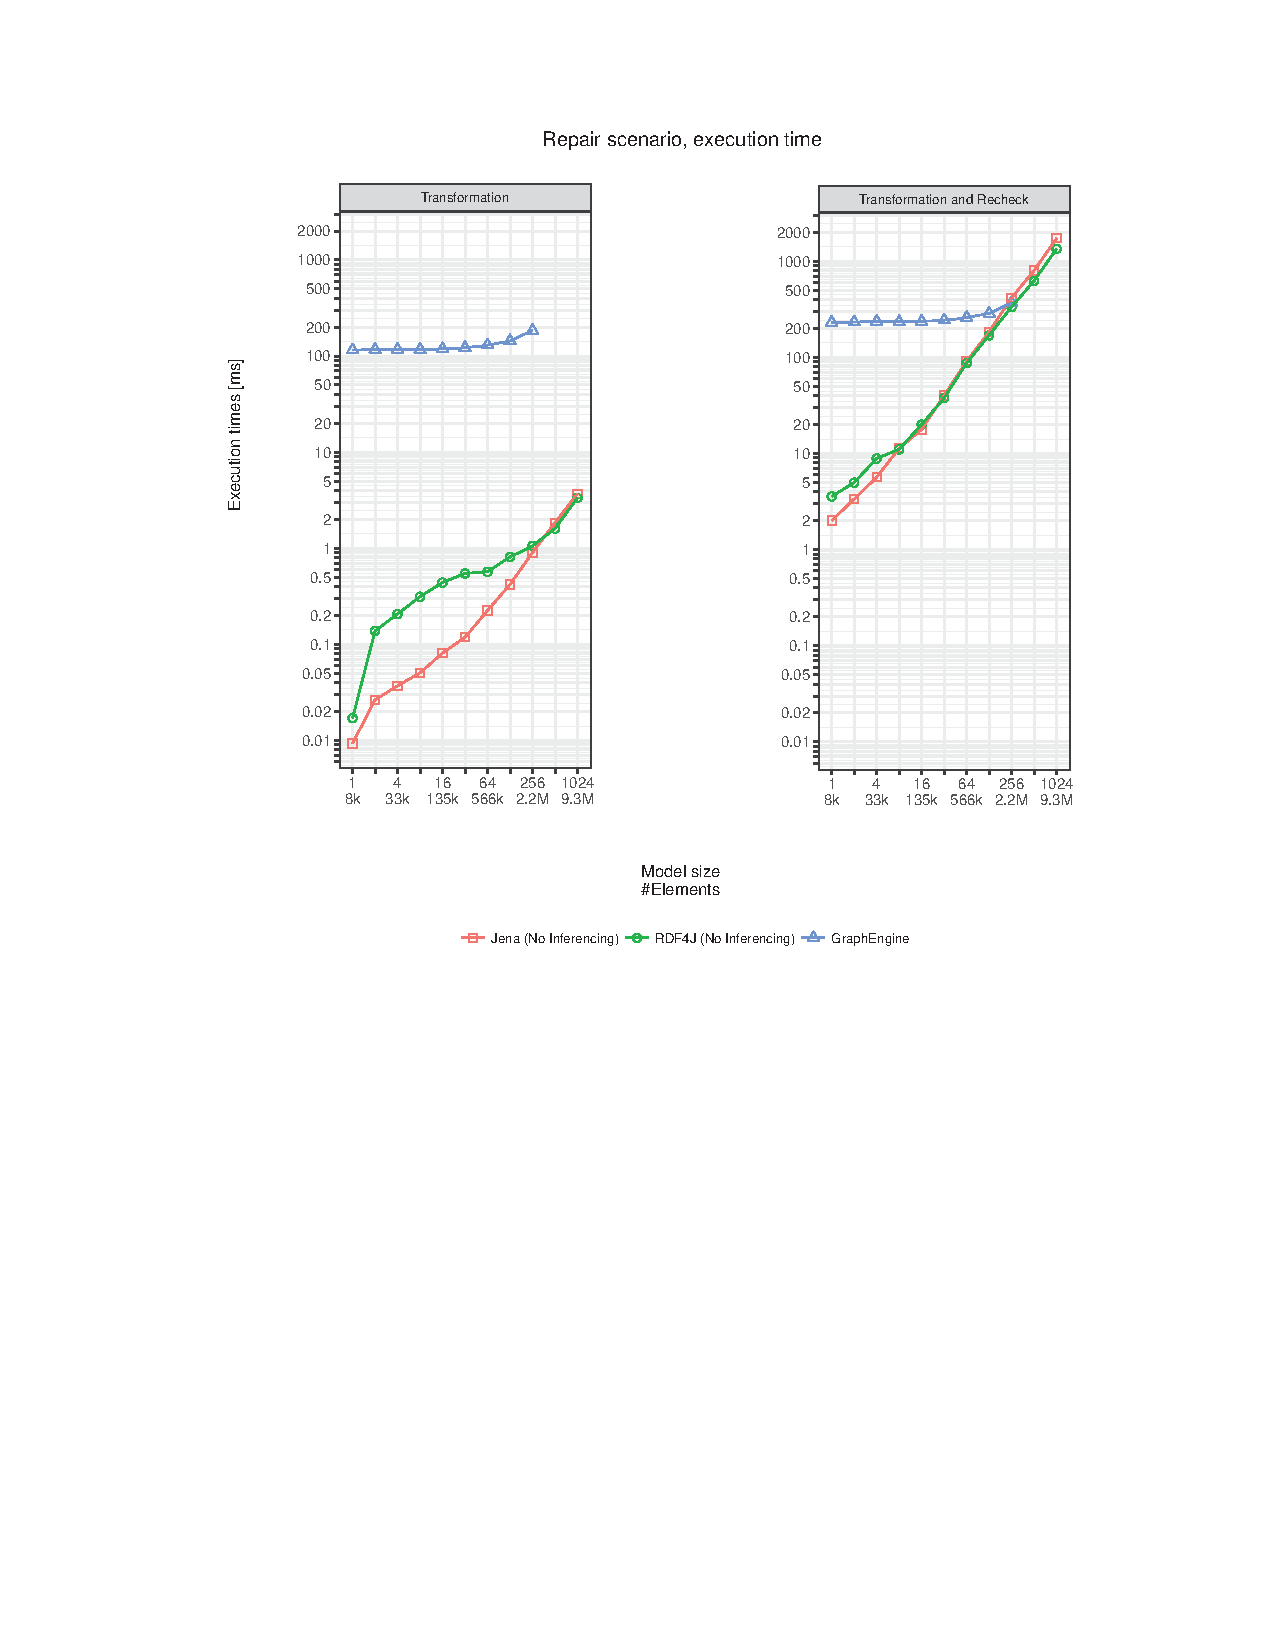
\includegraphics{figures/RouteSensor-times-Repair-Transformation-Recheck.pdf}
	\caption{A modelljavítás tesztelésének eredménye a \emph{RouteSensor} kényszer esetében.}
	\label{fig:RouteSensorRepairResultTransformation}
\end{figure}

%\section{A \emph{SwitchSet}-hez tartozó \emph{Inject} eredményeinek értékelése}
%
%A továbbiakban a \emph{SwitchSet} kényszer teljesülésének a feltételét vizsgáltuk. A modellbe a hibainjektálás és a javítás is a \emph{SwitchSet} kényszernek megfelelően történt. Az eredmények diagramja a \ref{fig:SwitchSetInjectResult} ábrán látható.
%
%A \emph{Read} fázisban a várakozásunknak megfelelően nem változott a teljesítmény. Azonban a \emph{RouteSensor}-hoz képest itt a Graph Engine csak eggyel kisebb modell esetében futott le elfogadható időn belül, az \emph{RDF4J} pedig eggyel nagyobbnál is.
%
%\pagebreak
%\begin{figure}[H]
%	\centering
%	\vspace*{-2cm}
%	\makebox[\linewidth]{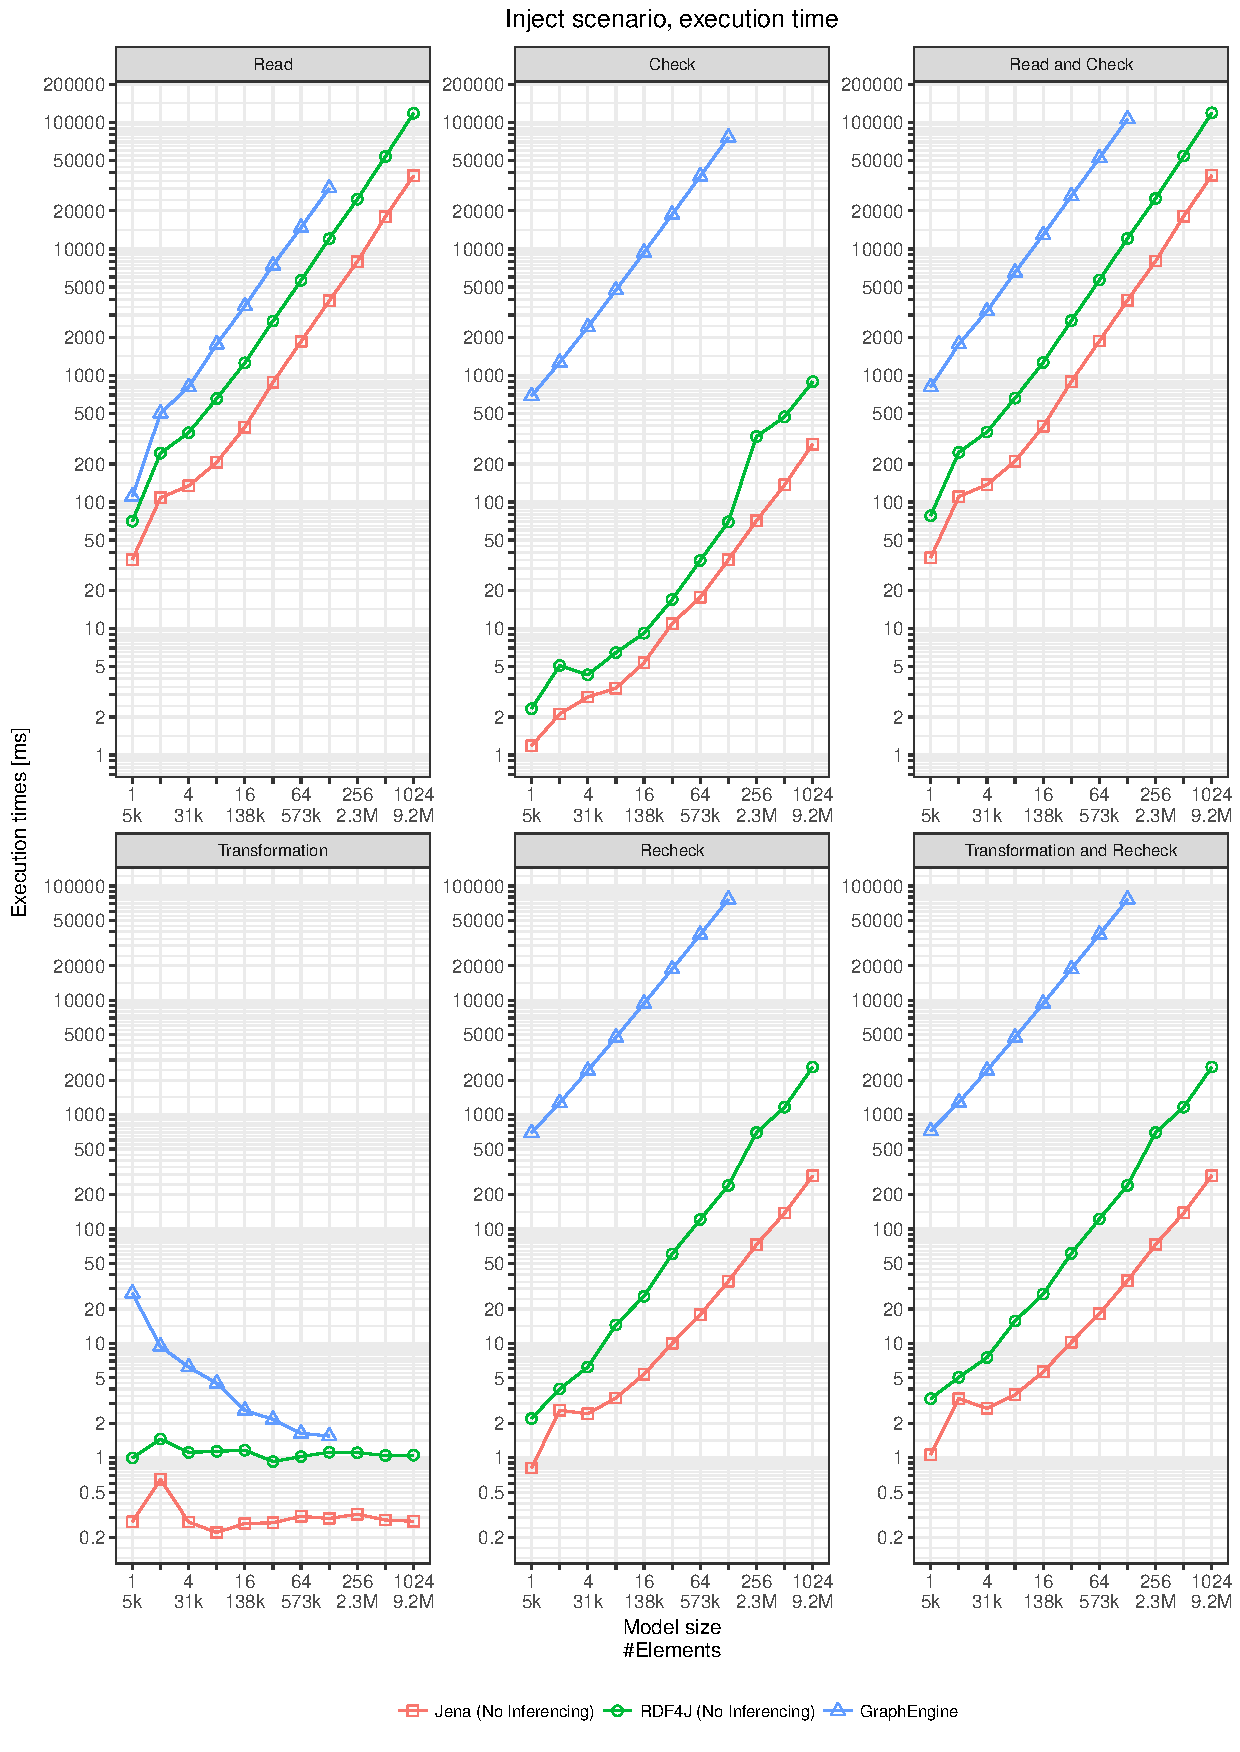
\includegraphics[width=1\linewidth]{figures/SwitchSet-times-Inject.pdf}}
%	\caption{A hibainjektálás tesztelésének futási idejeinek eredménye a \emph{SwitchSet} esetében.}
%	\label{fig:SwitchSetInjectResult}
%\end{figure}
%
%\subsubsection{Check és Recheck}
%
%A validációs fázisokban szemmel láthatóan elmarad a Graph Engine teljesítménye a többi eszközéhez képest. A futási idő bizonyos modelleknél több, mint 1000-szerese a másik két eszközének. Emellett a \emph{Jena} és az \emph{RDF4J} teljesítménye nőtt a \emph{RouteSensor} kényszer validációs teljesítményméréséhez képest, azonban a Graph Engine-é jelentős mértékben csökkent.
%
%Ennek az oka, hogy a \emph{SwitchSet} kényszerhez két \emph{LINQ} lekérdezés, ezáltal három \emph{foreach} ciklus van egymásba ágyazva, míg a \emph{RouteSensor}-nál csak egy \emph{LINQ} lekérdezés van. Az, hogy minden lekérdezés után az összes adatot el kell menteni a kliensoldali memóriába, emellett az adatbázishoz is rengeteg lekérdezést kell intézni a validációhoz, ezt az eredményt produkálta. Sokat javítana a teljesítményen, ha az adatbázishoz csak egy kérést kellene küldeni, azonban ez egyelőre nem megoldható, ugyanis több típusú gráfcsúcsot kell lekérdezni a kényszer validációjához.
%
%\subsubsection{Read and Check}
%
%A \emph{RouteSensor} kényszerhez tartozó \emph{Inject} méréssel ellentétben a \emph{Read and Check} szakaszban a validáció ideje a számottevőbb.
%
%\subsubsection{Transformation}
%
%A módosítás fázisban az \emph{RDF4J} és a \emph{Jena} teljesítménye kis kilengésekkel, konstans értéken marad a futási idő szempontjából. A Graph Engine esetében, hasonlóan a \emph{RouteSensor} módosításhoz képest, nagyobb modellekre rövidebb időértékeket mértünk, mint kisebbekre.
%
%\section{A \emph{SwitchSet}-hez tartozó \emph{Repair} eredményeinek értékelése}
%
%A \emph{SwitchSet} kényszer validációs teljesítménymérésének eredménye a beolvasás és validációs fázisokban megegyezik a hibainjektálásnál kapott eredményekkel. A módosítás fázisban a validációs szakasszal megegyező eredményt kaptunk. A módosításhoz először megkeresi azt, hogy hol található hiba, aztán kijavítja. Azonban azt megkeresni

\section{\emph{Performance Profiler}}

A \emph{Visual Studio} beépített \emph{Performance Profiler} funkciójával elemezni lehet egy \emph{.NET} platformon futó programot. Ezt arra használtuk, hogy megállapítsuk melyik az a függvényhívás, ahol a program a legtöbb időt tölti. Emellett lehetőség van azt is vizsgálni, hogy egy függvény hányszor hívódott meg. A \emph{Profiler} eredménye azt mutatta, hogy a \texttt{System.Collections.IEnumerator.MoveNext()} függvény végrehajtásával tölti a legtöbb időt a processzor. Ez egy \emph{LINQ} lekérdezés után az eredményeken való végigiterálásnál hívódik. Második helyen az \emph{TurtleParser} \texttt{Load()} metódusa áll, ami a \emph{dotNetRDF} könyvtár beolvasásért felelős függvénye.

%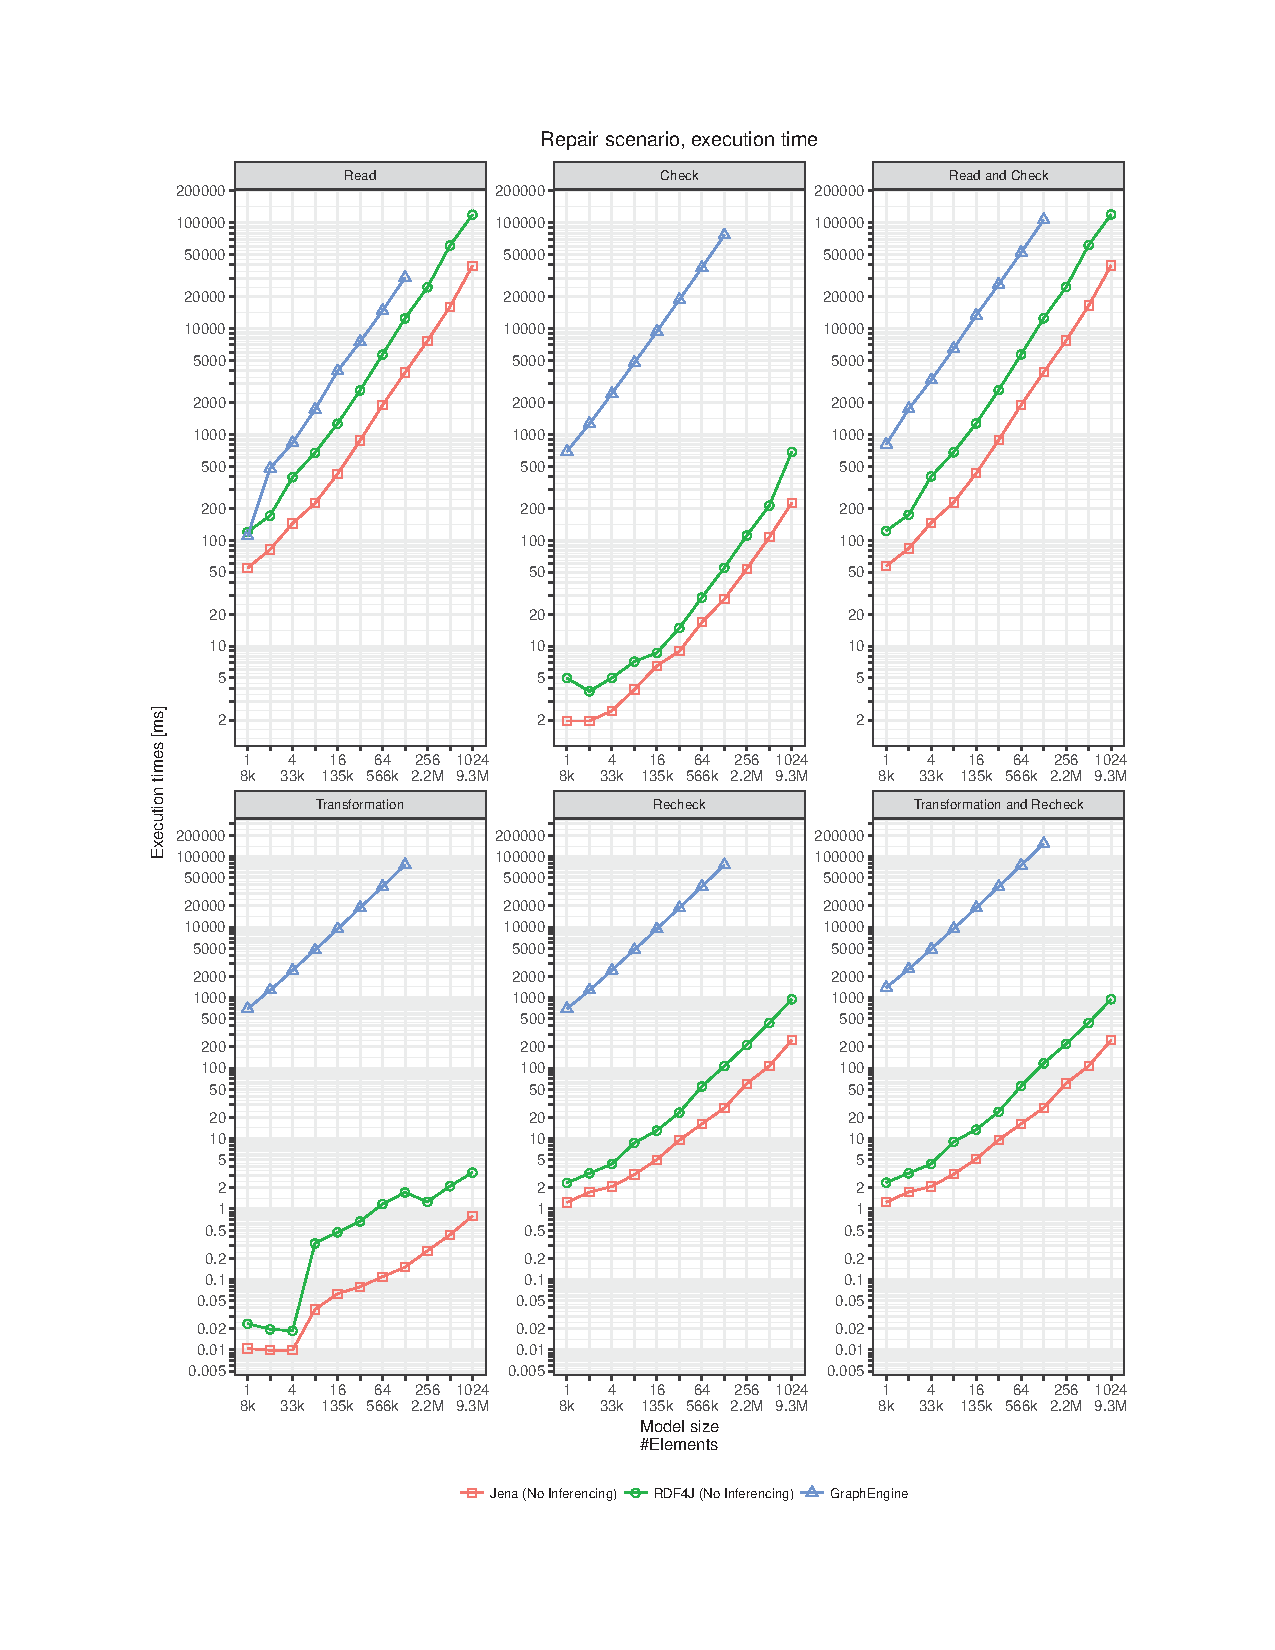
\includepdf[pagecommand={}]{figures/times-Repair.pdf}
%----------------------------------------------------------------------------
\chapter{Összefoglalás}
%----------------------------------------------------------------------------

%\include{content/latex-tools}
\include{content/thesis-format}
\include{content/template-usage}


% Acknowledgements
%~~~~~~~~~~~~~~~~~~~~~~~~~~~~~~~~~~~~~~~~~~~~~~~~~~~~~~~~~~~~~~~~~~~~~~~~~~~~~~~~~~~~~~
\include{content/acknowledgement}


% List of Figures, Tables
%~~~~~~~~~~~~~~~~~~~~~~~~~~~~~~~~~~~~~~~~~~~~~~~~~~~~~~~~~~~~~~~~~~~~~~~~~~~~~~~~~~~~~~
%\listoffigures\addcontentsline{toc}{chapter}{\abrakjegyzeke}
%\listoftables\addcontentsline{toc}{chapter}{\tablazatokjegyzeke}


% Bibliography
%~~~~~~~~~~~~~~~~~~~~~~~~~~~~~~~~~~~~~~~~~~~~~~~~~~~~~~~~~~~~~~~~~~~~~~~~~~~~~~~~~~~~~~
\bibliography{bib/mybib}
\addcontentsline{toc}{chapter}{\irodalomjegyzek}


% Appendix
%~~~~~~~~~~~~~~~~~~~~~~~~~~~~~~~~~~~~~~~~~~~~~~~~~~~~~~~~~~~~~~~~~~~~~~~~~~~~~~~~~~~~~~
\include{content/appendices}

%\label{page:last}
\end{document}
